\RequirePackage[l2tabu,orthodox]{nag}

% TODO: decide if one-sided/two-sided
%\documentclass[headsepline,footsepline,footinclude=false,fontsize=11pt,paper=a4,listof=totoc,bibliography=totoc,BCOR=12mm,DIV=12]{scrbook} % two-sided
\documentclass[headsepline,footsepline,footinclude=false,oneside,fontsize=11pt,paper=a4,listof=totoc,bibliography=totoc]{scrbook} % one-sided

% TODO: change citation style in settings
\PassOptionsToPackage{table,svgnames,dvipsnames}{xcolor}

\usepackage[utf8]{inputenc}
\usepackage[T1]{fontenc}
\usepackage[sc]{mathpazo}
\usepackage[ngerman,american]{babel}
\usepackage[autostyle]{csquotes}
\usepackage[%
  backend=biber,
  url=false,
  style=alphabetic,
  maxnames=4,
  minnames=3,
  maxbibnames=99,
  giveninits,
  uniquename=init]{biblatex} % TODO: adapt citation style
\usepackage{graphicx}
\usepackage{scrhack} % necessary for listings package
\usepackage{listings}
\usepackage{lstautogobble}
\usepackage{tikz}
\usepackage{pgfplots}
\usepackage{pgfplotstable}
\usepackage{booktabs}
\usepackage[final]{microtype}
\usepackage{caption}
\usepackage[]{acronym} % Package for acronyms
\usepackage{color,soul} % Package for highlighting
\usepackage[hidelinks]{hyperref} % hidelinks removes colored boxes around references and links
% Packages for EValuation questionnaire
\usepackage{wasysym}% provides \ocircle and \Box
\usepackage{enumitem}% easy control of topsep and leftmargin for lists
\usepackage{color}% used for background color
\usepackage{forloop}% used for \Qrating and \Qlines
\usepackage{ifthen}% used for \Qitem and \QItem
\usepackage{typearea}

\usepackage{comment}


\bibliography{bibliography}

\setkomafont{disposition}{\normalfont\bfseries} % use serif font for headings
\linespread{1.05} % adjust line spread for mathpazo font

% Add table of contents to PDF bookmarks
\BeforeTOCHead[toc]{{\cleardoublepage\pdfbookmark[0]{\contentsname}{toc}}}

% Define TUM corporate design colors
% Taken from http://portal.mytum.de/corporatedesign/index_print/vorlagen/index_farben
\definecolor{TUMBlue}{HTML}{0065BD}
\definecolor{TUMSecondaryBlue}{HTML}{005293}
\definecolor{TUMSecondaryBlue2}{HTML}{003359}
\definecolor{TUMBlack}{HTML}{000000}
\definecolor{TUMWhite}{HTML}{FFFFFF}
\definecolor{TUMDarkGray}{HTML}{333333}
\definecolor{TUMGray}{HTML}{808080}
\definecolor{TUMLightGray}{HTML}{CCCCC6}
\definecolor{TUMAccentGray}{HTML}{DAD7CB}
\definecolor{TUMAccentOrange}{HTML}{E37222}
\definecolor{TUMAccentGreen}{HTML}{A2AD00}
\definecolor{TUMAccentLightBlue}{HTML}{98C6EA}
\definecolor{TUMAccentBlue}{HTML}{64A0C8}

% Settings for pgfplots
\pgfplotsset{compat=newest}
\pgfplotsset{
  % For available color names, see http://www.latextemplates.com/svgnames-colors
  cycle list={TUMBlue\\TUMAccentOrange\\TUMAccentGreen\\TUMSecondaryBlue2\\TUMDarkGray\\},
}

% Settings for lstlistings
\lstset{%
  basicstyle=\ttfamily,
  columns=fullflexible,
  autogobble,
  keywordstyle=\bfseries\color{TUMBlue},
  stringstyle=\color{TUMAccentGreen}
}


% TODO: change thesis information
\newcommand*{\getUniversity}{Technische Universität München}
\newcommand*{\getFaculty}{Department of Informatics}
\newcommand*{\getTitle}{Automated documentation of Business Domain assignments and cloud application information from an application development pipeline}
\newcommand*{\getTitleGer}{Automatisierte Dokumentation von Business Domain Zuordnungen und Cloud Anwendungsinformationen aus einer Anwendungsentwicklungspipeline}
\newcommand*{\getAuthor}{Nicolás Corpancho Villasana}
\newcommand*{\getDoctype}{Master's Thesis in Information Systems}
\newcommand*{\getSupervisor}{Prof. Dr. Florian Matthes}
\newcommand*{\getAdvisor}{Martin Kleehaus}
\newcommand*{\getSubmissionDate}{15.02.2019}
\newcommand*{\getSubmissionLocation}{Munich}

\begin{document}

% Set page numbering to avoid "destination with the same identifier has been already used" warning for cover page.
% (see https://en.wikibooks.org/wiki/LaTeX/Hyperlinks#Problems_with_Links_and_Pages).
\pagenumbering{alph}
\begin{titlepage}
  % HACK for two-sided documents: ignore binding correction for cover page.
  % Adapted from Markus Kohm's KOMA-Script titlepage=firstiscover handling.
  % See http://mirrors.ctan.org/macros/latex/contrib/koma-script/scrkernel-title.dtx,
  % \maketitle macro.
  \oddsidemargin=\evensidemargin\relax
  \textwidth=\dimexpr\paperwidth-2\evensidemargin-2in\relax
  \hsize=\textwidth\relax

  \centering

  \IfFileExists{logos/tum.pdf}{%
    
\includegraphics[height=20mm]{logos/tum.pdf}
  }{%
    \vspace*{20mm}
  }

  \vspace{5mm}
  {\huge\MakeUppercase{\getFaculty{}}}\\

  \vspace{5mm}
  {\large\MakeUppercase{\getUniversity{}}}\\

  \vspace{20mm}
  {\Large \getDoctype{}}

  \vspace{15mm}
  {\huge\bfseries \getTitle{}}

  \vspace{15mm}
  {\LARGE \getAuthor{}}

  \IfFileExists{logos/faculty.pdf}{%
    \vfill{}
    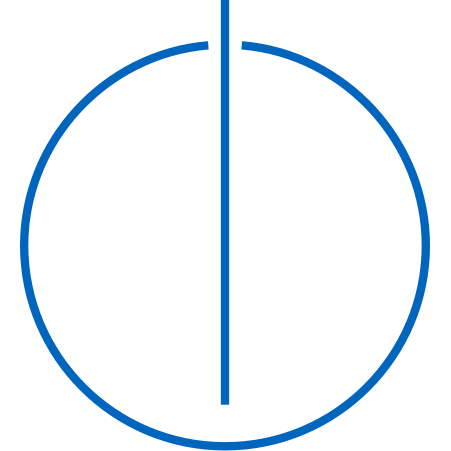
\includegraphics[height=20mm]{logos/faculty.pdf}
  }{}
\end{titlepage}


\frontmatter{}

\begin{titlepage}
  \centering

  \IfFileExists{logos/tum.pdf}{%
    
\includegraphics[height=20mm]{logos/tum.pdf}
  }{%
    \vspace*{20mm}
  }

  \vspace{5mm}
  {\huge\MakeUppercase{\getFaculty{}}}\\

  \vspace{5mm}
  {\large\MakeUppercase{\getUniversity{}}}\\

  \vspace{20mm}
  {\Large \getDoctype{}}

  \vspace{15mm}
  {\huge\bfseries \getTitle{}}

  \vspace{10mm}
  {\huge\bfseries \foreignlanguage{ngerman}{\getTitleGer{}}}

  \vspace{15mm}
  \begin{tabular}{l l}
    Author:          & \getAuthor{} \\
    Supervisor:      & \getSupervisor{} \\
    Advisor:         & \getAdvisor{} \\
    Submission Date: & \getSubmissionDate{} \\
  \end{tabular}

  \IfFileExists{logos/faculty.pdf}{%
    \vfill{}
    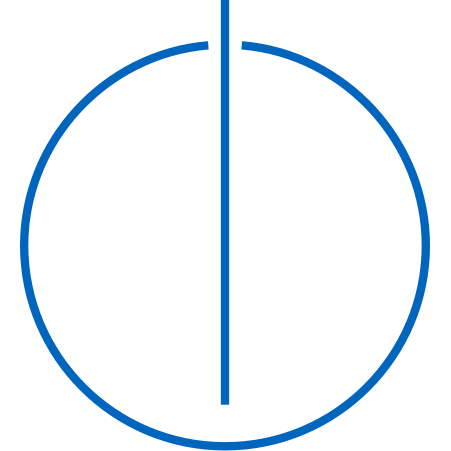
\includegraphics[height=20mm]{logos/faculty.pdf}
  }{}
\end{titlepage}

\thispagestyle{empty}
\vspace*{0.8\textheight}
\noindent
I confirm that this \MakeLowercase{\getDoctype{}} is my own work and I have documented all sources and material used.

\vspace{15mm}
\noindent
\getSubmissionLocation{}, \getSubmissionDate{} \hspace{50mm} \getAuthor{}

\cleardoublepage{}

\addcontentsline{toc}{chapter}{Acknowledgments}
\thispagestyle{empty}

\vspace*{20mm}

\begin{center}
{\usekomafont{section} Acknowledgments}
\end{center}

\vspace{10mm}


First of all I want to thank my advisor Martin Kleehaus for putting a lot of time and effort supporting me during the last months. His constructive feedback was of enormous value for the fulfillment of this thesis.

Furthermore, I want to thank Dr. Matheus Hauder and Martin Leichter for advising me on the industrial part of this work. Your support and feedback were also of immense value. 


I would like to thank Prof. Dr. Florian Matthes for giving me the opportunity to write my research topic at his chair and for his feedback.

In addition, I want to thank my team at the industry partner for making a collaboration possible, for participating in interviews and for the help during the last months.

Last but not least I would like to thank my family and friends for supporting me during the time of this work.

\cleardoublepage{}

\chapter{\abstractname}

%TODO: Abstract
% Abstract zu lang: um 2 Abschnitte kürzen, dafür Introduction länger?
Enterprise Architecture Management (EAM) has emerged to be a settled instrument to increase data quality, reduce IT costs and to reduce the error-prone effects of the process of the Enterprise Architecture information collection.

Although EAM has gained importance over more than a decade to improve the alignment of business with IT and transmit a holistic view of the entire organization along with its application landscape, this discipline has been shown to be more complex than expected.

One of the major challenges for an organization is the documentation of Enterprise Architecture (EA) information. Most of the EA documentation is still collected manually. The high number of applications within the application landscape coupled with data redundancy and the inconsistent data leads to a high complexity of EA documentation. This produces a time consuming and highly error-rated documentation and collection process of EA information. Maintaining and gathering information for the EA is (as well) a very expensive task.  The lack of governance is also a major challenge for EA itself. The absence of name conventions, standardized tools integration, continuous delivery and build pipelines, etc., adds to the complexity of a clear and transparent EA documentation.

Since one of the goals of EAM is to create a completely holistic view of the EA, it should integrate external sources, such as cloud services and other repositories.

This thesis will focus on the automated documentation of cloud applications information from an application development pipeline, and the business domain assignments based on the hypothesis that the automated documentation of EA cloud applications leads to a reduction of IT costs and effort, while increasing the data quality of EA information and data.

%TODO: Change. include static vs dynamic data to enrich data of ea tools. dynamic data for monitoring
In order to enhance a holistic view, the EA Tool can be enriched with dynamic data to enable a continuous process of monitoring application performance and infrastructure since the already available documented EA information is mostly static information and data coming from EA data sources.

\textbf{Keywords}: Enterprise Architecture Management, automated documentation, Business Domains, application development pipeline, cloud application information

\microtypesetup{protrusion=false}
\tableofcontents{}
\microtypesetup{protrusion=true}

\mainmatter{}
\microtypesetup{protrusion=false}
\listoffigures{}
\listoftables{}


\chapter*{List of Abbreviations}
\addcontentsline{toc}{chapter}{List of Abbreviations}

\begin{acronym}[ewuifbwejkbfjksbjkcbsdjcjkn3j]%set longest word for spacing

\acro{EA}[EA]{Enterprise Architecture}
\acro{EAM}[EAM]{Enterprise Architecture Management}


\end{acronym} % Abbreviations
% !TeX root = ../main.tex
% Add the above to each chapter to make compiling the PDF easier in some editors.

\chapter{Introduction}\label{chapter:introduction}

\section{Section}
Citation test~\parencite{latex}.

\subsection{Subsection}

See~\autoref{tab:sample}, \autoref{fig:sample-drawing}, \autoref{fig:sample-plot}, \autoref{fig:sample-listing}.

\begin{table}[htpb]
  \caption[Example table]{An example for a simple table.}\label{tab:sample}
  \centering
  \begin{tabular}{l l l l}
    \toprule
      A & B & C & D \\
    \midrule
      1 & 2 & 1 & 2 \\
      2 & 3 & 2 & 3 \\
    \bottomrule
  \end{tabular}
\end{table}

\begin{figure}[htpb]
  \centering
  % This should probably go into a file in figures/
  \begin{tikzpicture}[node distance=3cm]
    \node (R0) {$R_1$};
    \node (R1) [right of=R0] {$R_2$};
    \node (R2) [below of=R1] {$R_4$};
    \node (R3) [below of=R0] {$R_3$};
    \node (R4) [right of=R1] {$R_5$};

    \path[every node]
      (R0) edge (R1)
      (R0) edge (R3)
      (R3) edge (R2)
      (R2) edge (R1)
      (R1) edge (R4);
  \end{tikzpicture}
  \caption[Example drawing]{An example for a simple drawing.}\label{fig:sample-drawing}
\end{figure}

\begin{figure}[htpb]
  \centering

  \pgfplotstableset{col sep=&, row sep=\\}
  % This should probably go into a file in data/
  \pgfplotstableread{
    a & b    \\
    1 & 1000 \\
    2 & 1500 \\
    3 & 1600 \\
  }\exampleA
  \pgfplotstableread{
    a & b    \\
    1 & 1200 \\
    2 & 800 \\
    3 & 1400 \\
  }\exampleB
  % This should probably go into a file in figures/
  \begin{tikzpicture}
    \begin{axis}[
        ymin=0,
        legend style={legend pos=south east},
        grid,
        thick,
        ylabel=Y,
        xlabel=X
      ]
      \addplot table[x=a, y=b]{\exampleA};
      \addlegendentry{Example A};
      \addplot table[x=a, y=b]{\exampleB};
      \addlegendentry{Example B};
    \end{axis}
  \end{tikzpicture}
  \caption[Example plot]{An example for a simple plot.}\label{fig:sample-plot}
\end{figure}

\begin{figure}[htpb]
  \centering
  \begin{tabular}{c}
  \begin{lstlisting}[language=SQL]
    SELECT * FROM tbl WHERE tbl.str = "str"
  \end{lstlisting}
  \end{tabular}
  \caption[Example listing]{An example for a source code listing.}\label{fig:sample-listing}
\end{figure}

% !TeX root = ../main.tex
% Add the above to each chapter to make compiling the PDF easier in some editors.

\chapter{Foundations}\label{chapter:foundations}
\section{Enterprise Architecture Management} 

This chapter provides a theoretical overview of the discipline Enterprise Architecture Management. The most important concepts, related fields and its challenges related to EA are described in this chapter.

The aim is to describe the EAD process of organizations. This section will present the specific EA information sources and the key problems regarding the EAD. First EAM is defined and the stakeholders are mentioned. Then the different use cases of EAM will be presented. Since documenting the current state of the enterprise IT landscape is one of the uses cases, the different approaches found in the literature for automating that documentation process are presented.

%1.	Motivation. Um was geht es? In welchem Bereich befinden wir uns?
%2.	Problemstellung. Welche Herausforderungen leitest du aus (1) ab?
%3.	Lösungsziel. Welches Problem in (2) möchtest du genau lösen? 
%4.	Lösungsansatz. Wie möchtest du das Problem in (2) lösen?
%5.	Forschungsfragen. Welche Herausforderungen musst DU lösen um das Lösungsziel zu erreichen.
%6.	Evaluationsumgebung. In welche Umgebung kannst du deinen Lösungsansatz evaluieren? Welche Tools stehen %dir zur Verfügung?
%7.	Nächste Schritte.

\subsection{EAM Definition}
The term Enterprise Architecture Management is composed of three words: Enterprise, Architecture and Management.
According to ANSI/IEEE Std 1471-2000 architecture is defined as ‘the fundamental organization of a system, embodied in its components, their relationships to each other and the environment, and the principles governing its design and evolution.’
%Enterprise Architecture definition
Applying the previous mentioned definition to the context of enterprises, the EA refers to the fundamental organization of an enterprise, embodied in its components (e.g. organizational units, stakeholders, locations, business processes), their relationships to each other, the principles, methods and models that are used in the design and realization of the enterprise’s organizational structure.
\hl{(Buckl 2009)}
Additionally, the term management according to Mary Parker Follet refers to ‘the art of getting things done through people’ \hl{(van Aken 2005)}.
\hl{(Buckl 2009)}
\hl{(Jonkers 2006)}
In summary the three terms results to the following definition: EAM is promoted as an instrument to improve alignment of business and IT, ideally suggesting a common language and a framework across the company to determine  which business and technical domains, business processes, information systems and technical building blocks are used conveying a holistic view of the entire organization to realize cost savings potentials, and increase availability and fault tolerance.
\hl{(Hauder 2012)}
\hl{(Hanschke 2006)}

\subsection{EAM Stakeholders}
For a successful operation of EAM all relevant stakeholder groups need to be identified and involved.
When analyzing which stakeholder groups play a role in the organizations EAM initiative central functions, departments and project organizations as well as IT and external organizations have to be included. 
%The following questions can help for determine the stakeholder-groups: Who is the contracting authority? What concerns are associated with EAM? Who is the data supplier?
Figure \hl{XXX} shows an overview of the stakeholder groups that typically influence, have an interest or can benefit from EAM. \hl{(Hanschke ???)}
\begin{figure}[htpb]
  \centering
  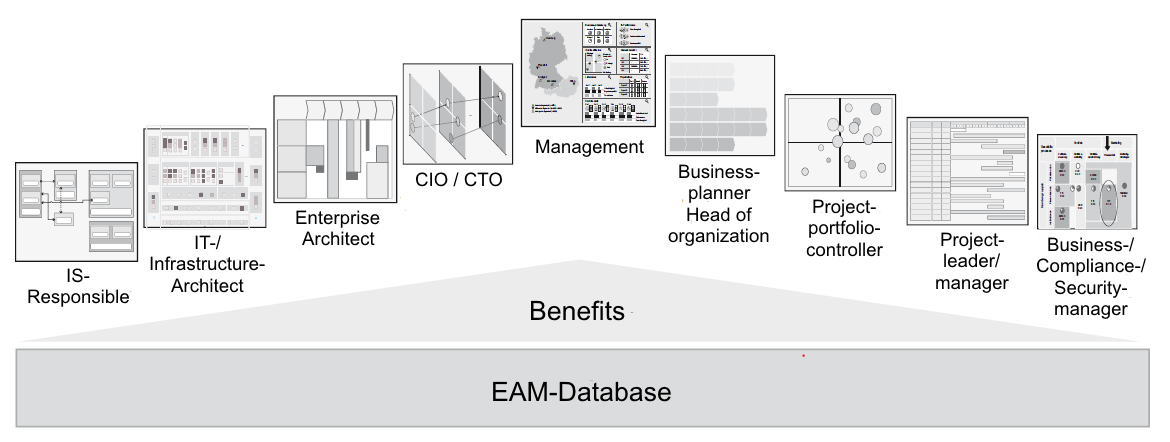
\includegraphics[width=0.8\textwidth]{figures/eam-stakeholder.png}
  \caption{ \hl{In Anlehnung an}Different stakeholder groups with interest in EAM~\parencite{Hanschke 2013}}
  \label{fig:Differet stakeholder groups with interenst in EAM}
\end{figure}

The following list shows stakeholder groups that are often involved in EAM initiatives in practice. The structuring is based on the TOGAF categories:\hl{(TOGAF Quelle)}
\begin{itemize}
    \item Corporate Functions
    \item End-User Organization
    \item Project Organization
    \item System Operations
    \item Externals
\end{itemize}

Not all categories are explained in detail. Only some stakeholder groups relevant for further sections of this work will be described briefly. These are named below and their tasks and EAM concerns are also explained. Some category mappings may vary by company. For example, enterprise architects are assigned to the stakeholder category IT.

\subsubsection{Corporate Functions}
\textbf{CIO (CTO)}: How are we performing on delivering our strategic goals? The CIO (CTO) covers the strategic corporate planning and definition of long-term target and framework requirements as well as planning and control systems and the corporate organization. The benefits of an EAM initiative is to ensure an optimization of the day-to-day business for the CIO (CTO) gathering a cross-company information report from the EAM database to provide the implementation of the corporate/enterprise goals.

\subsubsection{End-User Organization}
\textbf{Business manager}(including head of business units or areas and department heads): responsible for increasing the business IT alignment and further development of business and business architecture. Business managers endeavour to discover and remove technical redundancies and divisional differences in business processes and business capabilities and their IT support.

\subsubsection{Project Organization}
\textbf{Project leader or managers}: Responsible for the operative planning and control of a project. The expected benefits are reduced project preparation and input for project execution as well as input for operational planning and control of the project.
In addition to project managers, other stakeholder groups of a project organization may also benefit from EAM results. Examples include business analysts, software architects or solution architects. Solution architects often ensure the proper implementation of the development planning in projects through collaboration or review. 
%In collaboration with the project managers the channels of the offered %product is decided Which products will we offer via which channels? What %is the impact of making a change? What are the dependencies?

\subsubsection{System Operations}
\textbf{Enterprise Architects}: Main resposible for implementing and desgining and EAM initiative. Also in charge for the implementation of technical standards and principles and their use in the information system landscape and in the operational infrastructure as well as operational infrastructure development and the provision of SLAs at the operational infrastructure level.
%Which capabilities require investment to deliver our goals?


\subsubsection{Externals}
This category includes partners and suppliers, such as outsourcing service providers. The application of EAM to this category is the improvement of technical standards and specifications for the target development as input and framework conditions for services. The analysis of dependencies and effects of changes and the fulfillment of SLAs are also covered.

%Other stakeholder questions:
%Which applications are at risk from end-of-life technology?
%Which applications get replaces when?
%Which risks require mitigation? What are our greatest threats?

\subsection{EAM Use Cases}

% EA MetaModel
% use case areas
% Dependency management

In regard to the discipline EAM the use case types can be divided into two categories: operational and strategic use cases. This section will only list some key uses cases.

%Operational use cases
\subsubsection{Operational EAM use cases}
Operational use cases aim to support the current business cost-effectively and reliably with the help of IT, while continuously improving the IT support. The main challenges are: cost reduction, to reduce complexity of the IT landscape, the optimization of day-to-day business and identify risks. \hl{(Hanscke 2013)}.

As mentioned above only key uses cases are named in this section. Here is a list of some operational use cases:

%Metamodel hervorheben. Metamodel für abhängigkeiten
\textbf{Meta model as a common language}: Before gathering the EA data about the current state, an meta model of the architecture has to be defined, which describes the elements and relationships in between constituting the EA meta model to enable a common language across the organization. Collecting information from different layers requires the involvement of a multitude of stakeholders, e.g. business process owners, project managers, business architects, etc. Although working for the same organization, the definitions used by these stakeholders differ widely. This communication problem is often referred to as the communication gap between business and IT \hl{(Lankes 2008, Schekkerman 2004)}. This gap restricts adequate communication and collaboration in the EA management process.\hl{(Buckl et al. 2008)}. There are often more interactions between IT and business, as expected. To overcome this gap an EAM common language is needed. The resulting metamodel is used as the reference in the dialogue with the both parties.\hl{(Hanschke 2013)}

\textbf{EA Documentation}: In order to enable EAM and its life cycle, the current (as- is) state of the EA has to be documented. The different elements and layers covering business, organizational and infrastructure aspects have to be enclosed to provide a holistic view on the enterprise. The information gathered about the current situation, enables the planing for future states. Complementing the current and planned states of the EA an ideal target (to-be) state should be envisioned, which can be derived from the long-term vision of the enterprise. \hl{(Buckl et al. 2008)}. This use case will be described in detail in \subsectionautorefname{} Enterprise Architecture Documentation.

\textbf{Standardization and homogenization}: Definition of technical standards and monitoring of compliance and promotion of implementation. The goal of this use case is to reduce the IT complexity supporting the re-usability of proven technical building blocks. This increases the technical quality. The standardization and homogenization of technical standards concludes to a continuous cost reduction through the use of economies of scale and the bundling and reduction of the different know-how expertise.\hl{(Hanschke 2013)}

\textbf{Project portfolio management}: Creation of transparency about applications to optimize the support of business through IT and the planification of the roadmap for target architecture, ensuring the implementation of planned future development, IT consolidation and compliance in planning, prioritization, and overall governance and monitoring of the project portfolio. Through targeted management of project resources costs and also the IT complexity can be reduced.\hl{(Hanschke 2013)}

\textbf{Demand Management}: Planning and controlling the flow of strategic and operational business requirements for implementation through demand management. Demand Management translates the requirements between business and IT. As a bottleneck for the planning and control of the implementations of the business, it ensures that the technical goals and business requirements are adequately implemented.

%Strategic use cases
\subsubsection{Strategic EAM use cases}
Strategic use cases intent to improve systematically the development and strategic alignment of the different responsible. The main challenges are the setting of specifications and guarantee the compliance (EA Governance) and the progression of Business-Innovation and -Transformation.

\textbf{IS-Portfoliomanagement}: Identification of the potentials for the optimization in the IT landscape through the analysis of the architecture. One of the goals is to reduce the IT complexity through continuous IT consolidation and thus a sustainable reduction of IT costs. Another goal is to increase business IT alignment by evaluating the contribution of the IT to the business.

\textbf{Business-Transformation}: Standardization and homogenization of the future IT landscape
concerning the implementation of enterprise and IT strategy. The assurance of decisions can be ensured through the analysis of the dependencies and the effects of the IT landscape in relation to the business landscape.

According to the ANSI/IEEE Std 1471-2000 the main tasks of EAM are documentation (operational), communication (operational), and analysis of architectures (strategic). The following section will give a general outline of the enterprise architecture documentation.


\section{Enterprise Architecture Documentation} 

EAM begins with the documentation of the current state according to the defined EA metamodel to  derive future plans for an improved EA. Organizations endeavour with the documentation of the current state due to the complexity of enterprise architecture. This section will provide an overview of the enterprise architecture documentation process.

\subsection{Definition}

This first core product of EAM is the documentation of the current implementation of business processes, IT systems, and infrastructure (Schmidt and Buxmann 2010; Lankhorst et al. 2009; Kaisler et al. 2005; van der Raadt and van Vliet 2008). It needs to provide a current (PQ1a) and complete (PQ1b) view of the as-is architecture providing the right degree of detail (PQ1c) (Schmidt and Buxmann 2010; Foorthuis et al. 2010; Aier et al. 2011; Riege and Aier 2009; Winter and Fischer 2007; Aier and Schelp 2009; Bricknall et al. 2006; Schmidt and Buxmann 2010; Winter and Fischer 2007; Pulkkinen 2006). 

\subsection{Information Sources}
A survey conducted by \hl{Farwick} presents the major information sources for an EAD. This survey was done to provide an comprehensive analysis of possible information sources and their appropriateness for EA since research activities still seek to automate the data collection process.

The information sources correspond to the tools used by the participants of the survey. In addition, the participants also expressed their concerns regarding the EA relevant data delivered by the tool in respect of the following data properties in the EA context: actuality, completeness, correctness and granularity \hl{Farwick 2013}

\subsubsection{Network Scanners and Monitors}
%include source [4] of farwick 2013
The most common potential information source for an automated EAD are Network Scanners and Monitors. Operations teams often use these sources to monitor the infrastructure and its performance. As analyzed in the survey more than 60 percent of all organizations use Network Scanners.
Relevant data for network scanners are servers, applications and databases. However, the data gathered from this sources is too granular. The data can then not me mapped to the EA meta model. Nonetheless the correctness and the actuality of the data are considered positive. Since network scanners cannot cover all technologies the quality  of the collected data is worst of all information sources.

\subsubsection{Configuration Management Database}
Configuration Management Databases (CMDBs) are databases that store relevant information about hardware instances used in an organization's IT services and the relationships between those instances and the related incidents at an operational level.\hl{ITIL}
A CMDB should contain data about server, database and application instances. This data is mostly colleected and maintained manually. Same as with the network scanners, the data is too granular and organizations often use CMDBs for a strategic planning of EA since they provide all instances within the organization. \hl{farwick 2013}

\subsubsection{Project Portfolio Management tools}
Porjects are often modeled as a part of the EA metamodel. Project Portfolio Management (PPM) tools can trigger the EA maintenance process since a PPM tool often contains information about the start and end date, budget information and artifacts affected b the project. This data should be integrated with the EA tool since the aspect of project changes is a central aspect of EAM. \hl{farwick 2013}
The actuality and completeness of the data is in most cases maintained regularly but it depends on project management of the organizations. On the pther hand it is difficult to decide which project is actually architecture relevant so the granularity is affected by that.

\subsubsection{Enterprise Service Bus}
%Include dependendy mngt in Use cases
There is no common definition for Enterprise Service Buses (ESB) but in most cases ESBs act like a layer on top of the applications allowing the communication between them. The messages sent by the applications can be routed through the ESB which makes the communication possible. The transformation of the messages facilities the connection of different applications to use their own native message formats. This layer enables the integration of third party and legacy
systems. This leads to a total dependency of the IT landscape. \hl{Falko 2007}
The analysis and optimization of dependencies between applications is also a central aspect of the EAM discipline. This is the reason why the actuality and correctness of the data quality attributes received very positive evaluations. However, the integration of an ESB and transformation and mapping of the communication between the applications is very challenging. This affected the answers about the data granularity. \hl{Farwick 2013}

\subsubsection{Change Management Tool}
Change Management Tool are used to improve the procedure of implementing changes in the
IT-landscape. Frequently the tools are maintained manually and thus do not cover all changes. This is reflected in the answers for data actuality, correctness and completeness. The negative
outcome for the granularity also implies that the data is difficult to map to EA metamodel.
Nevertheless Change Management tools can trigger a manual action to keep the EA tool up-to-date.

\subsubsection{License Management Tools}
License Management Tools provide an overview of acquired software licenses. The information provided by the tool is the number of installations, number of users, costs, acquisition date and type and duration of licenses. The information was seen as EA relevant. Actuality, completeness, and correctness had a good outcome, whereas granularity has a moderated outcome. A large number of participants of the survey could not value the data quality attribute of a license management tool. This indicates that EA stakeholders do not always access these tools and therefore the integration depends on the usage.

\subsubsection{Excel Import/ File Import}
Many of the participants of the survey pointed out that the import of file, specially importing excel-sheets is a potential information sources since many of the organizations still rely on the usage of Microsoft Excel sheets for keeping data.

\subsubsection{External Sources: Cloud Services}

The usage of cloud services was mentioned frequently for collecting infrastructure data. \hl{(Farwick 2013 - Information Sources)} Apart from documenting traditional hardware, cloud infrastructure information needs to be collected in an EA tool. Cloud-based environments are much more volatile than traditional environments. Therefore, it is important to integrate EA tools with cloud infrastructure to enable tracking of changes occurring in the cloud. \hl{(Farwick 2010 - Towards)}


\subsection{EA Documentation Challenges}

Nowadays the documentation process of the EA is performed in most of the organizations manually. This leads to many challenges:

\subsubsection{Data challenges}

Maintenance of EA Models
High Complexity: Manual collection of EA data
High number of applications
Data redundancy
Inconsistent data
leads to: High error rate documenting and collecting EA information
Time consuming collection of information
Expensive tasks

\subsubsection{EA Governance}
% bafin regulatorische anforderungen?

% Agil: jedes Team benutzt irgendwelche Tools vs EA/IT Governance: Vorgaben von richtlinien

% Annahme: Da lack of governance: Toolchain "Integration" in die Development pipeline für die Dokumentation

\subsubsection{Tooling}


\subsubsection{Fast changing environment}

% Welche Lösungsansätze gibt es bereits
% Comparisson der Ansätze
% Comments: show IT, wie wird das erfasst?

\section{Technology trends influencing EA}

XXX

\subsection{Agile development and Continuous Delivery and Integration}

CD, CI
Short life cycles

\subsubsection{Definition}

\subsection{Modularization}
%Decomposition of legacy systems into modules / microservices
\subsubsection{Definition}

\subsection{Cloud Computing}
% Argumentation für Migration in die Cloud. Focus on core competences
% Cloud Computing als Theoretical Background?

Migration of legacy systems

\subsection{Monitoring}

\subsubsection{Definition}
Cloud computing is a model for enabling universal, on-demand and convenient network access to a shared pool of configurable computing resources (e.g., servers, applications, storage, networks and services) that can be quickly provisioned and released with little to no management effort or service provider interaction”.
\hl{(Isaac Odun-Ayo 2018)}
\hl{(The NIST Definition of Cloud Computing. NIST Special Publication 800-145 2011.)}



\section{Automated Enterprise Architecture Documentation}

This work will target automation of the documentation use case  trying to improve the strategic analysis with the help of application monitoring as a result of the automated EAD. First, the technology trends covered in the section beforehand are outlined regarding the impact they have on EAD. Then the different solution approaches found in the literature review are presented.

\subsection{Technology Trends in automated EAD} 

\subsection{Literature solution approaches}

\subsection{}
\chapter{Related work}\label{chapter:relatedwork}

This work will target the automation of the documentation use case trying to improve the strategic analysis with the help of application monitoring as a result of the automated EAD. First this chapter will present different solution approaches related to automated EAD. Then the different proposed solutions will be compared and evaluated. 

%Hauder 2012 - Challenges for automated enterprise architecture documentation
Hauder et al. \cite{Hauder2012} describes the EA documentation process as very time consuming, error-prone and a process that requires a lot of manual effort. Inspired by these challenges Hauder examines the further challenges for an automated EAD investigating model transformations from various information sources, conducted a survey among 123 EA practitioners and incorporated a literature review. The discovered problems among EAD were grouped into four categories. The main challenge of the first category data is the appropriate selection of a relevant EA information source and the data quality retrieved. The second category identified is transformation. It reports the problems regarding the alignment and maintenance of data from diverse information sources to a central repository. The third category business and organization deals with the question of the added value of an automated process and what the impact to the organizational structure is. The last category describes the challenges related to the tool. 

%Farwick 2013 - Enterprise Architecture Documentation: Empirical Analysis of Information Sources for Automation
A survey conducted by Farwick et al. \cite{Farwick2013} reveals more details about the  status quo of EA documentation processes in organizations, which information sources can be used to obtain relevant EA information, what integration problems exist for these information sources and what data quality attributes like data actuality,  data completeness, data correctness and the granularity level of the data, can be expected from them. The survey presents a list with the possible information sources and the expected data quality attributes. The survey declares that the gap between the retrieved data and the EA model prevents enterprises for automating the documentation process due to different granularity levels and the difficulties mapping the data to the EA model.

%Roth 2013 - Enterprise Architecture Documentation: Current Practices and Future Directions 
Roth et al. \cite{Roth2013} reaffirms the struggle of the organizations regarding the EA documentation process with an empirical evaluation on the application of this process. The survey implies the EAD of 140 organizations to validate the challenges mentioned by Hauder et al. \cite{Hauder2012} and by Farwick et al. \cite{Farwick2013} The work derives future research directions from the findings and gives an overview of the currently applied techniques in EAD. 
%These are compared to literature to validate the hypotheses regarding EAD.


%Microservices Architecture Enables DevOp
% Welche Lösungsansätze gibt es bereits
% Comparisson der Ansätze
% Comments: show IT, wie wird das erfasst?
\section{Literature approaches}

\subsubsection{Farwick 2010}
%TowardsLivingLandscapeModels:AutomatedIntegrationofInfrastructureCloud inEnterpriseArchitectureManagement

Farwick et al. \cite{Farwick2010} proposes in his work that cloud infrastructure should be documented in an EA model to increase the understanding between the cloud infrastructure in relation to other business information systems and finally to the overall business goals. The purpose of the publication is to present an approach how to consolidate runtime information of different information sources such as cloud environments to an EAM view. The work presents a conceptual approach and a prototypical implementation using the open-source cloud infrastructure Eucalyptus as well as the open-source EAM tool Iteraplan. The automated approach of Farwick et al. integrates different information sources in a central model, which updates the model, verifies the information and pushes the new information to the EAM tool. The publication proposes as a future work taking into consideration the integration of other cloud service models like PaaS and SaaS for the usage of generic APIs for standardization purposes. The synchronization problems with other information sources and the development of the central model and the metamodel are presented as future research due to the intensive work of the installation of agents for monitoring the different information sources. 

\subsubsection{Buschle  2012}
%Automating Enterprise Architecture Documentation using an Enterprise Service Bus
The presented approach of Buschle et al. \cite{Buschle2012} examines a specific Enterprise Service Bus (ESB) in an enterprise for interlinking business applications and processes as information sources. The transformation rules for the data are used to apply an automated EA documentation. The evaluation of the approach was carried out with a productive ESB in an enterprise in the fashion industry. 

\subsubsection{Holm  2014}
%Automatic data collection for enterprise architecture models
Holm et al. \cite{Holm2014} recommends using a network scanner for the automated process of data collection for producing EA models based on the IT infrastructure of enterprises. Manual effort is still required to make the models completely valuable. The results were evaluated empirically and demonstrate an accurate outcome with little effort.

\subsubsection{Välja 2015}
%  A requirements based approach for automating enterprise it architecture modeling using multiple data sources
The work of Välja et al. \cite{Valja2015} describes how to automate the process of EA modeling. The information is retrieved from different data sources using common data processing methods. The work shows that challenges of manual modeling can be overcome and data quality issues can be solved. The approach shows that it is possible to create automatically enterprise IT architecture models that are timely and scaleable. \cite{Valja2015}

\subsubsection{Farwick 2015}
%A situational method for semiautomated enterprise architecture documentation
The work presents a semi-automated approach for documenting EA with the respective tool. It focuses on the adaptability of the metamodel at runtime, the integration of different EA information sources and the versatility and scalability of the visualizations of the tool. The tool was presented as a prototype in the original article and has progressed to a commercial product called Txture.\cite{Farwick2015a}

\subsubsection{Johnson 2016}
%Automatic probabilistic enterprise IT architecture modeling: A dynamic bayesian networks approach
Johnson et al. \cite{Johnson2016} introduces an approach to automate the modeling of EA. The modeling process is seen as a probabilistic state estimation problem. Therefore a Dynamic Bayesian Networks is used to solve the estimation problem. The suggested approach proposes extensions to the model of ArchiMate. Using a Dynamic Bayesian Network detecting uncertainties surrounding the IT landscape becomes possible. Filtering the relevant information from the irrelevant remains still a challenge in this approach and it is therefore seen as a topic for further studies.

\subsubsection{Landthaler 2018}
% A Machine Learning Based Approach to Application Landscape Documentation
Landthaler et al. \cite{Landthaler2018} presents a machine-learning based approach for detecting and identifying the ArchiMate metamodel entity "application component" in the IT landscape of the enterprise. The presented approach discovers and classifies binary strings of application executables on target machines. The main challenge is that the binary strings of executables differ depending on the devices. That means that the same binary string is different for the same application version, device type and OS version. Evaluating the data reflected to major problems of this approach: the many-label nature of the classification problem and limited existence of sparse classification of the results.
The advantage of this approach is that all executable binaries are discovered independently from their name or installation path. 
For further evaluation of the approach it is necessary to examine the work on a heterogeneous environment. That means different operations systems and different versions of the same application to improve the classification of the applications based on related functionality.\cite{Landthaler2018}

\subsubsection{Bogner 2016}
% Towards Integrating Microservices with Adaptable Enterprise Architecture
Bogner et al. \cite{Bogner2016} examines methodologies to integrate the growing amount of small structures like microservices, Internet of Things and mobility services that are emerging in today's IT environments. Micro-granular architectures increase the degree of heterogeneity of enterprise's IT landscapes and thus hinder classical EAM approaches to deal with the diversity and distribution presented in the architecture landscapes. The work enlarge EA methodologies by extending earliest reference metamodels with elements for a more adaptable models and EA-mini-descriptions. The EA-mini-descriptions provide an adaptable metamodel for the microservices and the descriptions can be grouped to form superordinated entities. It also proposes that an EA approach should integrate small structures to enable a holistic view and should be flexible. The main intention of the paper is to identify adaptability issues of microservice architectures and to present a different approach than classical EAM approaches. The development of a prototype and the evaluation and validation of the results in practical use cases is requested as future research.

\section{Derivation of requirements}\label{subsection:derivationofrequirements}

%Derivation of requirements for automated approach
% 1. Dynamic metamodel
% 2. Integrate runtime KPIs
% 3. Different information sources
% 4. Tranformations problems
% 5. Integrate Cloud (PaaS and SaaS)
In the previous section the different approaches were presented. These cover various aspects of EAD and have different outlooks for future works. From the introduced approaches and their respective problems, requirements can be derived for future solutions regarding automated EAD. The following table presents the derived requirements:

\begin{table}[htpb]
  \caption[Automated EAD requirements derived from literature approaches]{Automated EAD requirements derived from literature approaches}\label{tab:literaturerequirements}
  \centering
  \begin{tabular}{l l l}
    \toprule
      Id & Requirement & Source\\
    \midrule
      RL1 & Integration of different information sources. &\cite{Farwick2010}\cite{Farwick2015}\cite{Bogner2016}\cite{Johnson2016}\cite{Landthaler2018}\\
      RL2 & Dynamic metamodel &\cite{Hauder2012}\cite{Farwick2013}\cite{Roth2013}\cite{Farwick2010}\cite{Buschle2012}\cite{Holm2014}\cite{Valja2015}\cite{Bogner2016}\\
      RL3 & Business added value &\cite{Hauder2012}\cite{Roth2013}\cite{Farwick2010}\\
      RL4 & Tool support &\cite{Hauder2012}\cite{Roth2013}\cite{Holm2014}\cite{Farwick2015}\\
      RL5 & Integration of cloud environments (PaaS and SaaS) &\cite{Farwick2010}\cite{Farwick2015}\cite{Bogner2016}\\
      RL6 & Integration of runtime KPIs &\cite{Farwick2010}\cite{Farwick2015}\cite{Bogner2016}\\
    \bottomrule
  \end{tabular}
\end{table}

%Involvement of data owners for the maintenance of imported EA information

\textbf{RL1}: Most of the mentioned works propose the integration of different information sources. The survey conducted by Farwick et al. \cite{Farwick2013} shows that organizations use different information sources and/or see the information sources as potential EA relevant data sources. The findings are affirmed by the published approaches.
Regarding the data of the various sources, there are several data aspects that need to be covered. The integration presents the following data challenges:

\begin{table}[htpb]
  \caption[Data challenges in the integration of different information sources]{Data challenges in the integration of different information sources}\label{tab:data-challenges}
  \centering
  \begin{tabular}{l l l}
    \toprule
      Id & Challenge & Source\\
    \midrule
      DC1 & Data granularity &\cite{Hauder2012}\cite{Farwick2013}\cite{Roth2013}\cite{Holm2014}\cite{Valja2015}\\
      DC2 & Data actuality &\cite{Hauder2012}\cite{Farwick2013}\cite{Roth2013}\cite{Holm2014}\cite{Valja2015}\cite{Johnson2016}\cite{Landthaler2018}\cite{Bogner2016}\\
      DC3 & Data completeness &\cite{Hauder2012}\cite{Farwick2013}\cite{Roth2013}\cite{Holm2014}\cite{Valja2015}\\
      DC4 & Data correctness &\cite{Hauder2012}\cite{Farwick2013}\cite{Roth2013}\cite{Holm2014}\cite{Valja2015}\cite{Johnson2016}\cite{Landthaler2018}\\
    \bottomrule
  \end{tabular}
\end{table}

\textbf{DC1}: Data granularity describes detail level of information. This challenge affects the mapping of the different model since the granularity and abstraction level of the models is different. If the data too fine-grained it is not relevant stakeholder of EA.
%T2 en challenges for Automated Enterprise Architecture Documentation

\textbf{DC2}: Data actuality defines how up to date is the information contained in the information source. To ensure the actuality of the data the EA repository requires an detection of changes. The same applies to the different information sources. The changes in the real world need to trigger a maintenance of the EA relevant data.
%empirial analysis
%challenges of automated entepris...

\textbf{DC3} and \textbf{DC4}: Data completeness and Data correctness are further quality attributes of the gathered data.They refers to the amount of relevant data  and accuracy covered by the information source.

The above mentioned data challenges lead to an EA model maintenance. As describes by the approaches the underlying model needs to be flexible.

\textbf{RL2}: As mentioned before data is retrieved from numerous information sources. The collected information varies regarding the data content and granularity levels (DC1). Therefore a transformation of the data to the target metamodel is required. 
%This requirement includes several aspects regarding the data collected from the information sources. The data sources use different models. 
The transformation of the data should convert the model of the source to the target model. Duplicate EA elements or attributes should also be identified and removed from the target model (DC4). The various models are also diverse regarding the granularity levels of the models (DC1). This is why the target model for the collected data should be dynamic. This means that it has to be able to allow different granularity levels since the different stakeholder may consider the retrieved information as EA relevant.

\textbf{RL3}: The business added value of an automated EAD is not considered as enough regarding the return of investment. The initial investment required for an automated EAD is to large and requires too much effort. The data owners of the information sources need to be involved in the process of the information collection and need to maintain the imported EA information. This is also seen as a challenge according to the survey conducted by Hauder et al. \cite{Hauder2012}\cite{Matthes2008}\cite{Matthes2014}

\textbf{RL4}: Tool support is also mentioned as a requirement in the related approaches for an automated EAD. The main challenge regarding the tooling aspect is that the majority of the tools does not support an integration of different information sources due to the lack of a public API. Therefore, Iteraplan is used in most of the approaches as the EA Tool since it offers a public API to integrate various data sources. \cite{Matthes2008}\cite{Matthes2014} Another problem regarding the EA Tools is the absence of customizing visualizations for analyzing the collected data. \cite{Hauder2012}\cite{Matthes2008}\cite{Matthes2014}

\textbf{RL5}: Cloud infrastructures are emerging in many organizations. \cite{Bogner2016}
%Bogner 
According to that the integration of cloud environments need to be coupled to EAM. %Farwick,
Cloud environments supports an enterprise in many ways. Enterprises can host the applications in a public or a private cloud and these also vary in the service offering. Cloud can be contracted as IaaS, PaaS and/or SaaS. Similar to traditional EA relevant information sources these options of cloud need to be documented. The integration of different cloud environments present the same data challenges as mentioned in table~\ref{tab:data-challenges}. Some of the approaches have proposed an installation of agents \cite{Landthaler2018}\cite{Farwick2010} in the underlying infrastructure to retrieve information from installed applications. Considering the usage of PaaS and SaaS as a cloud infrastructure the generic cloud API can make the installation of these agents obsolete.
%Farwick
Another advantage of cloud infrastructure is that it also offers the possibility to integrate runtime information of the applications which leads to the next requirement: R6 - Integration of runtime KPIs.

\textbf{RL6}: The integration of runtime KPIs is also proposed in the approaches found during the literature reasearch. \cite{Frank2009}\cite{Farwick2010}
%As already mentioned, enhancing EA models with KPIs can improve the analysis of EAM. 
% An integration of runtime KPIs can therefore be derived from literature. 
An enhancement of runtime KPIs improves the actuality of the collected data (DC2). In also increases the data completeness and correctness. \cite{Frank2009}\cite{Farwick2010}\cite{Hauder2012}

\section{Summary}

This section will give an overview of the topics covered by the different approaches presented in literature. 

\begin{table}[htpb]
  \caption[Topics covered by the literature approaches]{Topics covered by the literature approaches}\label{tab:literature-summary}
  \centering
  \begin{tabular}{l l l l l}
    \toprule
      Year & Author & CD & CC & AM\\
    \midrule
      2012 & Hauder et al. &   &   & X\\
      2013 & Farwick et al. &   & X & X\\
      2013 & Roth et al. &   &   &  \\
      2010 & Farwick et al. &   & X &  \\
      2012 & Buschle et al. &   &   &  \\
      2014 & Holm et al. &   &   &  \\
      2015 & Välja et al. &   &   &  \\
      2016 & Farwick et al. & X & X & X\\
      2016 & Johnson et al. &   &   &  \\
      2018 & Landthaler et al. &   &   &  \\
      2016 & Bogner et al. & X & X & X\\
    \bottomrule
  \end{tabular}
\end{table}

Table~\ref{tab:literature-summary} shows that current research endeavours lack in integrating cloud aspects (PaaS and SaaS) with its respecting structures such as microservices for automated EA documentation. \cite{Buschle2012} Also agile methodologies and continuous delivery and integration are not taken into consideration when it comes to the automation of the EAD. New approaches can be derived from the topics that are not covered and the requirements derived from the already existing approaches.

The approach that will be presented in the next chapter will integrate the EAD process within the application development pipeline to enable a continuous automated EAD. The approach will also include an automated documentation of business domain assignments by extracting the business domains from the PPM tool during the application development pipeline.
The integration of an automated EAD within a continuous delivery pipeline has not been covered in the literature. In addition to that, cloud environments like PaaS and SaaS will be integrated by the approach of this work for an automated EAD of cloud applications.



\chapter{Solution approach of an automated EAD process}\label{chapter:evaluation}


\section{...}

%eampc: priorisierung von migrationen.
%eampc: aggregated architecture of enteprise oder cloud applikationen

% !TeX root = ../main.tex
% Add the above to each chapter to make compiling the PDF easier in some editors.

\chapter{Prototype implementation}\label{chapter:prototype implementation}

\section{...} 


% Jira Skript Ausnahmen

% anpassung in groovy. githublink
% httpSecurity.csrf().disable();













\chapter{Evaluation}\label{chapter:evaluation}

% !TeX root = ../main.tex
% Add the above to each chapter to make compiling the PDF easier in some editors.
%\chapter{Case study}\label{chapter:EA documentation in an insurance company} 
% IST-Analyse
% EA documentation in an insurance company

This chapter introduces in the first section the evaluation of the implemented prototype in a case study. The second section will explain the factors that influence the IT landscape of the insurance company. These are divided into internal and external factors. In the next section~\ref{section:asislandscape} the IT landscape is explained. The current method of the EA documentation process in the insurance company is explained. The EAD process was conducted during this  master-thesis.
In the following section~\ref{section:targetitlandscape} the target IT landscape will be described.
At the end of this chapter in section~\ref{section:derivedrequirements}, the derived requirements to automated the EA relevant information collection process will be presented to introduce the new approach for an automated EAD.

\section{Case Study Design}\label{section:casestudy}

The case study was conducted according to the research methodology for software engineering from Per Runeson. \hl{Per Runeson, 2008}

\subsection{Case study objectives}\label{subsection:casestudyobjectives}

This case will identify the current practice and the challenges regarding the EAD process in a german insurance company. The case study evaluated the suggested solution of an automated EAD process and its prototype derived from the requirements found out during the literature research. To improve the solution the prototype was evaluated in the company to derive further requirements for an automated EAD.

\subsection{Case study definition}\label{subsection:casestudyobjectives}

The subject of this case study is a international insurance company based in Munich. The investigation in this case will mainly focus on the Enteprise Architecture Documentation process within the company. To understand the process, the study will take a look at the IT landscape to retrieve information how the EA relevant components interact with each other and what factors influence the IT landscape. This will give an overview to find out why the enterprise is documenting EA relevant information in that way.

\subsection{Case study methodology}\label{subsection:casestudymethodology}

\subsubsection{Research questions -  what to know?}
%How  to  assign  the  application  landscape  to  business  domains?
%How  to  obtain  EA  relevant  information  from  the  runtime  behaviour  ofcloud-based environments?
%How to automate the assignment process with an integrated toolchain?
%How  does  a  prototype  implementation  of  the  automated  documentationprocess of cloud applications look like?
The research questions that are going to be answered are mentioned in ~\ref{section:researchquestions}.
RQ1 and RQ3 are relevant for the case study. The aim is to see if the questions can be answered during the case study to derive requirements to improve the EAD.

\subsubsection{Methods — how to collect data?}

As mentioned by Runeson et al. \hl{Per Runeson, 2008} the following information sources can be used to collect data:

\begin{itemize}
    \item Different data sources
    \item Archival data
    \item Interviews
\end{itemize}

%Archival data refers to, for example, meeting minutes, documents from different development phases, organizational charts, financial records, and previously collected measurements in an organization

During the case study a literature research was conducted to derive challenges and requirements from literature to be able to compare the information to the of current situation the company.

An analysis of the archived data of the company was executed during the thesis in order to gain more knowledge about the IT landscape, the reasons of the current documentation process, projects changing the landscape and its documentation and what the enterprise expects to be improved or even automated.

To retrieve more information informal and semi-structured interviews were conducted.The interviews were divided into 2 parts. The first part explained the motivation and the objectives of the thesis. The motivation introduced a brief overview of the scope of the thesis and the objectives includes the research questions to be answered. The second part of the interview consisted of questions regarding the findings during the research of the current situation.

\section{Factors influencing the IT landscape}\label{section:influencingfactors}

This section will describe the influencing factors that have an impact on the IT landscape of the german insurance company. To understand the IT landscape an overview of the main influencing factors is presented. First, the internal factors are explained. Secondly, the external factors such as regulations will be mentioned. Finally, EA documentation process will be described. 

\subsection{External factors}\label{subsection:externalinfluencingfactors}

The section will describe the most important external factors that change the IT landscape of the enterprise and thus have an impact on the EAD. There are three regulations that mainly influence the EAM. The first regulation is the General Data Protection Regulation (GDPR). The second factor affecting the IT landscape is the VAIT Regulation. The last regulation influencing the IT landscape is the international standard ISO 22301.

\subsubsection{General Data Protection Regulation}

The General Data Protection Regulation (GDPR) is a European Data Protection Regulation that enforces all member states of the European Union to harmonize data privacy laws. The GDPR is related to processing of personal data. It assures fundamental rights of  persons, especially the right to the protection of personal data.

\subsubsection{VAIT Regulation}

The regulation "Versicherungsaufsichtliche Anforderungen an die IT" (engl. "Insurance supervisory requirements for IT") (VAIT) affects the IT of insurance companies with headquarters in Germany. The use of information technology (IT) in companies, including IT services offered by IT service providers, is of central importance to insurance companies and pension funds. The circular letter published in the context of the regulation mentioned contains information on the interpretation of the regulations on business organization in the Insurance Supervision Act  (in german "Versicherungsaufsichtsgesetz") (VAG) insofar as they relate to the technical organizational equipment of the companies. It makes these regulations binding for Federal Financial Supervisory Authority (in german "Bundesanstalt für Finanzdienstleistungsaufsicht") (BaFin), thereby ensuring consistent application to all companies and groups. The circular letter provides a flexible and practical framework, in particular for the management of IT resources, information risk management and information security management. \hl{Rundschreiben VAIT}

The main requirement affecting the EAD is the IT operations requirement. The IT operation must implement the fulfillment of the requirements resulting from the implementation of the business strategy as well as the IT-supported business processes. The components of the IT systems and their relationships to each other should be managed appropriately and the inventory information collected should be updated regularly and on an ad hoc basis. The stock information includes in particular: Inventory and purpose of the components of the IT systems with the relevant configuration information, location of the components of the IT systems, compilation of the relevant information on warranties and other support contracts (possibly linking), information on the expiration date of the support period of the components of the IT systems, accepted Period of unavailability of the IT systems and the maximum tolerable data loss. \hl{Rundschreiben VAIT}

\subsubsection{ISO 22301}

The ISO 22301 standard represents the latest international policy for Business Continuity Management (BCM) and was released in 2012. Its objective is to assist in the reduction of business interruptions due to unforeseen emergencies. This is the norm an update of the standards ISO 31000 and ISO 27001. It is considered a universal standard in the the sense that they apply to companies of all sizes and regardless of the used technologies.

To ensure the reduction of unforeseen emergencies an IT emergency system should be introduced to act as a a holistic management system. That includes monitoring and regular review of the IT landscape. These two aspects enable one of the main components of the standard execution: the Business Impact Analysis. 

The Business Impact Analysis (BIA) is a complex task that includes important corporate resources as a precautionary measure: specialists, executives and corporate management. The analysis includes the collection and identification of processes and functions,
the required resources such as staff, but also hardware resources like IT facilities, buildings, warehouses with their technical equipment. The analysis also include dependencies on IT processes, the definition of the core processes and impacts and recovery times.
\hl{Springer Notfallplan in Kommunikationsnetzen}

\subsection{Internal concerns}\label{subsection:internalinfluencingfactors}

The internal factors presented in the following paragraphs are mainly the drivers that have an impact on the IT landscape of the enterprise.

\subsubsection{Main business system}

The main legacy system of the insurance company has developed over time into a legacy system. Application components were built to connect new systems or application to enable a communication between those. The added layers, components and adapters led to an not transparent and not maintainable legacy system. To improve the transparency of the legacy system the enterprise decomposed the system into modules to gain information about the dependencies to other applications and/or systems.

\subsubsection{Business Continuity Management}

Driven by the ISO standard 22301 the german insurance company of this case study is also obliged to fulfill this regulation through a BCM project. The company is exposed to increasing risks that endanger the continuous and timely provision of its services to the customer. Contributing to this are various developments and trends in society and the economy, such as growing globalization, increasing networking, centralization, automation, outsourcing.
Due to the increasing complexity of business processes and their increasing dependence on information technology and external service providers, events such as fire, flood or the failure of information technology and external service providers or personnel can have a major impact.

The Business Continuity Management (BCM) is a management process with the aim of early identification of serious risks for the enterprise, which endanger the existence, and to establish measures against them. In order to ensure the viability and thus the existence of the company, appropriate preventive measures must be taken, which on the one hand increase the robustness and reliability of the business processes and on the other hand enable rapid and targeted response in an emergency or crisis.

The goal of the BCM is to ensure that important business processes are not or only temporarily interrupted, even in critical situations, and that the economic existence of the enterprise remains secured even in the event of a major loss event (crisis cases require separate consideration). A holistic view is therefore crucial. Consider all aspects that are required to continue critical business processes when a claim event occurs, not just the Information Technology resource. IT emergency management is part of the BCM.
Critical business processes in the sense of emergency management means "time-critical", so that this process requires a faster resumption of activity, otherwise a high level of damage can be expected. The high damage can result from financial losses, violations of laws or contracts, from image damage or other damage scenarios.
A business process classified as "uncritical" does not mean that it is unimportant to the enterprise, but merely that it has a lower priority in recovery.

\subsubsection{Decommissioning project}

The goal of the decommissioning project is to withdraw traditional data centers from active service to mainly to reduce costs. The decommission of applications or systems can be executed have different reasons. The first reason is to decommission systems due to lack of support available or the purpose to remove old legacy systems. The data of the removed system has to be migrated to the new system. The another reason for decommissioning systems is to withdraw traditional data centers from active service. The efficient redistribution of IT resources can lead to migrations of systems from one data center to another to reduce the amount of running data centers and consequently reduce the costs of running data centers. The other approach of migrating applications to withdraw servers is the migration to the cloud. The elasticity of the cloud enables the efficient use of computational efficiently and has as a consequence that traditional server can be withdrawn.

\subsubsection{Cloud migration project}
%TODO: include sources for this subsection: Chen 2015,  Odun-Ayo 2018
The migration to the cloud of the IT infrastructure is a central and strategic issue. The expansion of the IT architecture, including cloud solutions, forms the basis for digitization and increases the productivity and efficiency of IT processes. The migration improves the availability and scalability of IT services, thereby increasing the growth potential of all IT structures. The duration of the total migration amounts to an estimated 4 years and is divided into quarterly projects. The migrated applications / Minimum Viable Products (MVP) are put into production at the end of the quarter and put into line.

The arguments for migrating to the cloud are divided into two aspects. The arguments covering the first aspect of operations are:
\begin{itemize}
    \item Performance and Availability: OpenShift and CloudFoundry are proven solutions that are used in many large organizations and designed for high availability.
    \item Scalability: OpenShift and CloudFoundry enables fast and easily scalable automation of applications based on demand and load.
    \item Cost Efficiency: Moving from traditional virtualization technology to container technology will bring better utilization of existing resources and, in the long run, cost savings.
    \item Security: OpenShift and CloudFoundry provide easy deployment of security patches for platform and applications. The updates can be imported without downtime for the end user. Both providers also offer easy deployment of security patches for platform and applications. The updates can be imported without downtime for the end user.
\end{itemize}
The following migration arguments cover the second aspect of application development:
\begin{itemize}
    \item Developer Satisfaction: Developers can leverage cutting edge technologies to build innovative solutions.
    \item Developer Efficiency: CloudFoundry is designed as a self-service platform. Developers get more freedom in a well-defined framework to get to their destination faster.
\end{itemize}

The project objectives are:
\begin{itemize}
    \item Full application migration without interruption to ongoing operations (24x7 applications, sales, support and night jobs). These means the technical migration of more than 400 applications.
    \item Create a migration blue print and best practices for dealing with the new infrastructure.
    \item Creation of the migration framework including half / tools to carry out the migration
    \item Supplementing the operational concept for post-migration operations. This means the monitoring and error analysis of the migrated applications after the production has been set for the duration of the project.
\end{itemize}

The project does not include the migration of fat clients and \hl{non-insurance-owned} applications.

\section{AS-IS IT landscape}\label{section:asislandscape}

This section will described the IT landscape of the company. The following picture shows the main components of the IT landscape.

\begin{figure}[htpb]
  \centering
  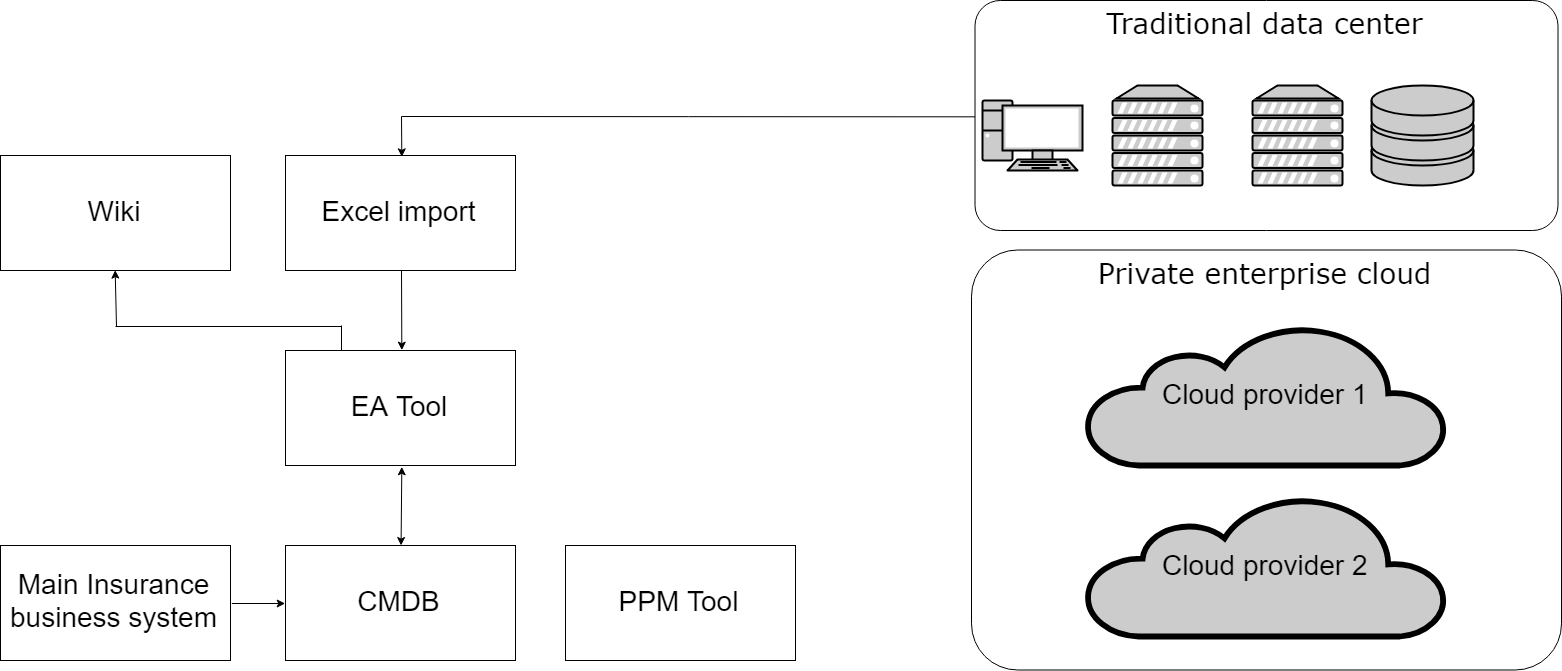
\includegraphics[width=0.8\textwidth]{figures/as-is-it-landscape.png}
  \caption{ AS-IS IT landscape~\parencite{Corpancho Villasana 2018}}
  \label{fig:AS-IS IT landscape}
\end{figure}

The company consists of two environments: the traditional environment which contains traditional data center hardware and its private cloud infrastructure which is divided into two different cloud service providers. The first cloud infrastructure service provider is OpenShift and the second provider is Pivotal's CloudFoundry.

The traditional data centers host the legacy systems of the company and all other kind of applications.

OpenShift is a container platform. The PaaS provider OpenShift offers the possibility to deploy docker containers to its platform and enables the orchestration by Kubernetes. \hl{OpenShift}

CloudFoundry (CF) is an open source, multi-cloud application platform as a service. Similar to Openshift, CF has a container-based architecture which also enables the deployment of applications written in any programming language.

The main components of the IT landscape in regard to EAm are the EA tool, the CMDB, the PPM tool, a service-oriented architecture (SOA) repository, the Wiki s a collaboration software program and the main business system. As shown in the picture above the enterprise uses Iteraplan as their EA tool. %AMUR?
The SOA repository is used for managing services such as WSDLs and XML schema definitions, access rights, information related to the service level agreements and transactional operations of the services. \hl{Enterprise SOA Buch} 
%Enterprise SOA: Service-oriented Architecture Best Practices By Dirk Krafzig, Karl Banke, Dirk Slama
Relevant for the EAM are the other repositories depicted in the picture. Other repositories include change management tools, license management tools, etc.

\subsection{Current EA documentation}\label{subsection:currentead}

The EAD integrates several tools as shown in figure \hl{XXX}. 
\subsubsection{Excel import}

The first EA documentation process was driven by the external mentioned ISO 22301 standard. The enterprise decided to collect the information about the IT landscape. The usage of Microsoft Excel sheets for keeping data is still important for enterprises since many organizations still rely on them for information storing.\hl{}

Initially the systems or applications that are critical for the business were documented. This was mainly driven by the BCM project and the BIA of IT failures. Ensuring that important business process are not interrupted and have no economic impact to the company is essential that the enterprise remains secure. For this initiative a team was created to retrieve this information. The documentation process was done fully manually. Therefore the document containing the information was inconsistent and contained redundant information.

The continuation of the project is mainly driven by the VAIT regulation since enterprise will have to have a fully application inventory.

\subsubsection{Integration of the CMDB}
% Pasarlo a current EA docu?
Due to the BCM regulation mentioned in section~\ref{section:internalinfluencingfactors}, an integration between the EA tool and the CMDB was implemented. The EA tool integrates data from the CMDB. The application developed for the integration retrieved data from the CMDB and imports the data to the EA tool in regular intervals. The import is was unidirectional. Only Business Services were imported from the CMDB. No infrastructure data was integrated into the EA tool. The import did not analyze the data, meaning that if the imported data was redundant there was no merge conflict solved. The integration was developed to improve these challenges. The Integration on the CMDB contains now a conflict solution and harmonizes the redundant imported applications with a unique identifier. The import mechanism also differentiates between a flag set in the CMDB metamodel to import the business services as an application or a technical components. This differentiation is done because in the CMDB everything was modeled as a business service.

This integration was the pilot integration project for information sources to the existing EA tool. Further integrations of different information sources will be implemented due to the successful development of this integration.

The main business system of the enterpise was initially documented in the CMDB. For that reason the information about the main business system was retrieved via the CMDB to the EA tool.

%Semi automated?
The integration of the CMDB to the EA tool is semi-automated since the information of the CMDB was also retrieved manually.

\subsubsection{Export to Wiki}

The export of the collected data in the EA tool was mainly driven by the integration of the CMDB. The goal of the data export to the Wiki was to analyze and evaluate the data of the EA tool. 

Enterprise Wikis enhances sharing and collaboration of employees knowledge. The employees can easily edit the wikis content and provide their knowledge to the information center. The unstructured information can contain file attachments, multimedia content and allows the interlinkage of wiki pages. Referencing EA relevant information such as documents is supported by wikis. To link this references wikis are more appropriate than an EA tool.\hl{Fiedler 2013}

To enable the collaboration and knowledge sharing of the employees knowledge a Wiki was integrated into the IT landscape. A wiki page is created for each application of the EA tool. This enables to collect more data than the metamodel of the EA tool allows. The wiki page contains several characteristics of an application. Some of the extended characteristics of an application are architectural decision, users, architectural diagrams, decommissioning information driven by the decommission concern, operational manual and other notes regarding the application.

\subsubsection{Cloud integration}

As we can see in picture \hl{XXX} there is no integration of the applications running on the cloud-based environments. There is no defined process of the EAD of applications deployed to the cloud.

\subsubsection{PPM Tool integration}

As figure \hl{XXX} shows, there is no integration of a PPM Tool.

\section{Target IT landscape}\label{section:targetitlandscape}

This section will explain the target IT landscape of the company. The target IT landscape is mainly driven by the concerns. The following picture shows the target IT landscape.

\begin{figure}[htpb]
  \centering
  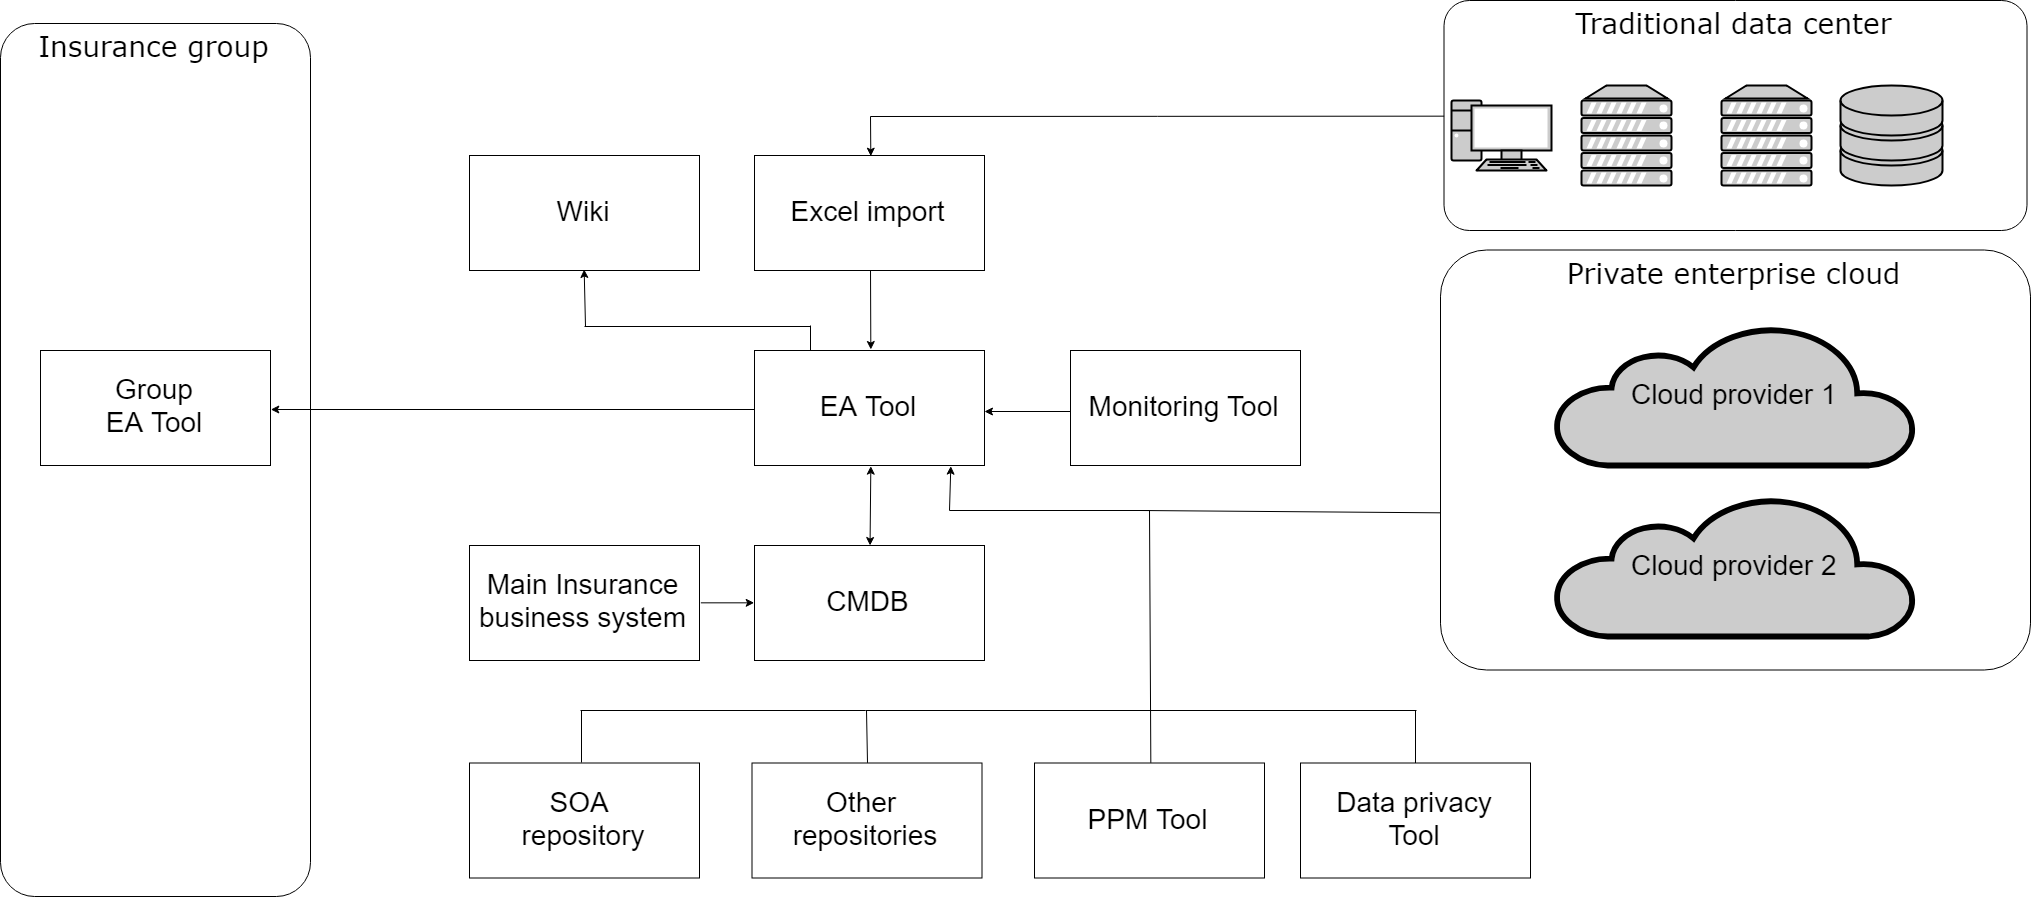
\includegraphics[width=0.8\textwidth]{figures/target-it-landscape.png}
  \caption{ Target IT landscape~\parencite{Corpancho Villasana 2018}}
  \label{fig:Target IT landscape}
\end{figure}

\subsubsection{Integration of data privacy tool}
%Amur für datenschutz
Driven by the GDPR the enterprise has developed a tool which contains a list of applications that are related to this regulation. Therefore an integration of this tool is planned in order to have this specific information in the EA tool.

\subsubsection{Integration of service-oriented architecture repositories}

An integration of a service-oriented architecture (SOA) repository enables the enterprise to include inventories of the web services in a SOA repository to the EA tool. Therefore an integration is intended.

\subsubsection{Integration of other repositories}
The enterprise goal of the enterprise is to interlink different tools containing different EA relevant information. This goal enables a federated architecture to allow information sharing between different data sources. Therefore it will also integrate other repositories such as license management tools and change management tools.

\subsubsection{Integration of the PPM tool}
The main goal of the integration of a PPM Tool is to enable a mapping between the projects and the applications or systems in the enterprise. The EA tool in place contains in its metamodel the entity "project". This allows an integration of the PPM tool to the existing EA tool. The projects of the PPM tool are imported into the EA tools as the entity "project". A manual mapping between the projects and applications is then still required. This EAD process of projects can be seen as semi-automated.

\subsubsection{Integration to the group EA tool}

The insurance company is divided into several subsidiaries around the world.The VAIT regulation is applied to every german insurance company. The german insurance company has its headquarters in Germany so the regulation implies an IT inventory for every subsidiary of the insurance company. Therefore every operating entity (subsidiary) has to export the EA information to the Group entity.

\subsubsection{Cloud integration}

As shown in picture \hl{XXX} the applications running on the cloud-based environments will be integrated to the EA tool. The main driver for this integration is the VAIT regulation. As mentioned in the regulation, an insurance company has to be able to deliver an application inventory of the IT landscape. That includes also applications running on private enterprise clouds. 

In the context of the cloud migration project a new defined process for the deployment of the new developed applications was introduced. The major goal of this defined process is to establish a standardized process for agile teams. The process is divided into a build process and a deployment process.

\begin{figure}[htpb]
  \centering
  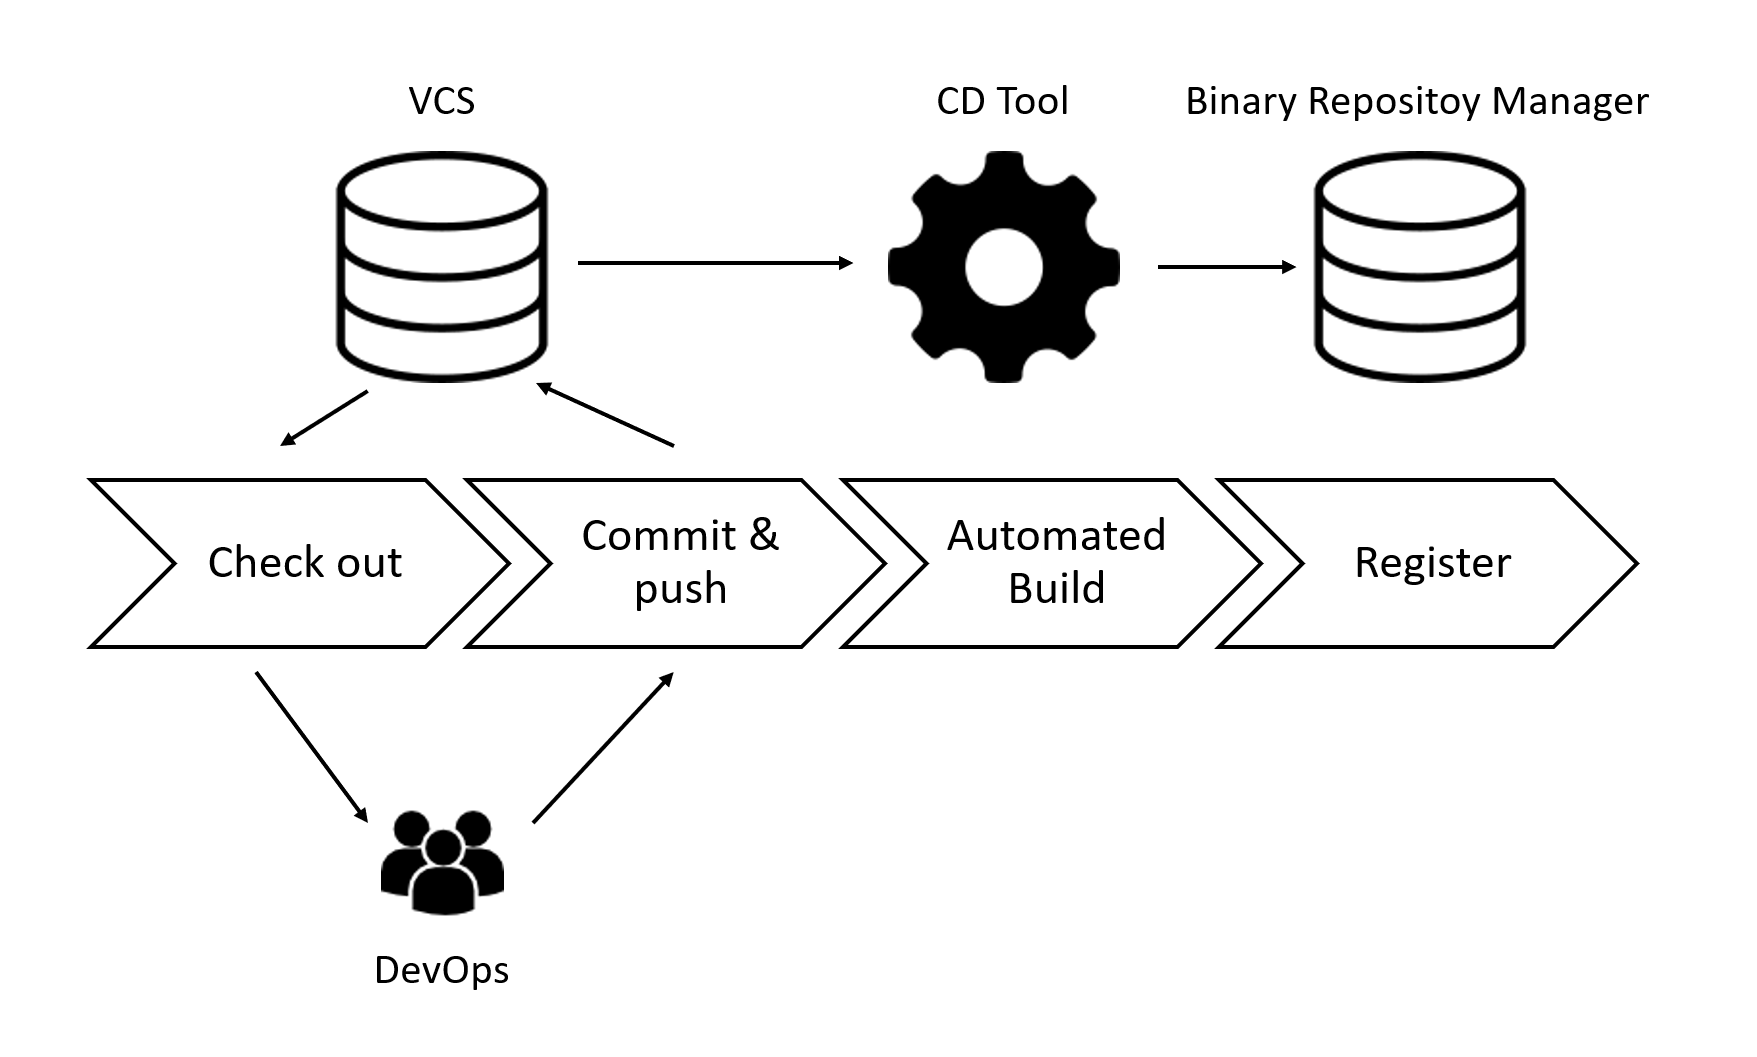
\includegraphics[width=0.8\textwidth]{figures/build-process.PNG}
  \caption{ Build process~\parencite{Corpancho Villasana 2018}}
  \label{fig:Build-process}
\end{figure}

The build process is shown in picture \hl{XXX}. The DevOps team first checks out the latest state of the code from the version control service (VCS). After developing the team commits and pushes the new state back to the VCS repository. The CD tool is constantly monitoring the repository to track changes in the code. If new changes are tracked, the CD tool automatically builds an artifact of the repository and registers the artifact into the binary repository manager tool. That means the built artifact is hosted in the tools and can be downloaded from it.

\begin{figure}[htpb]
  \centering
  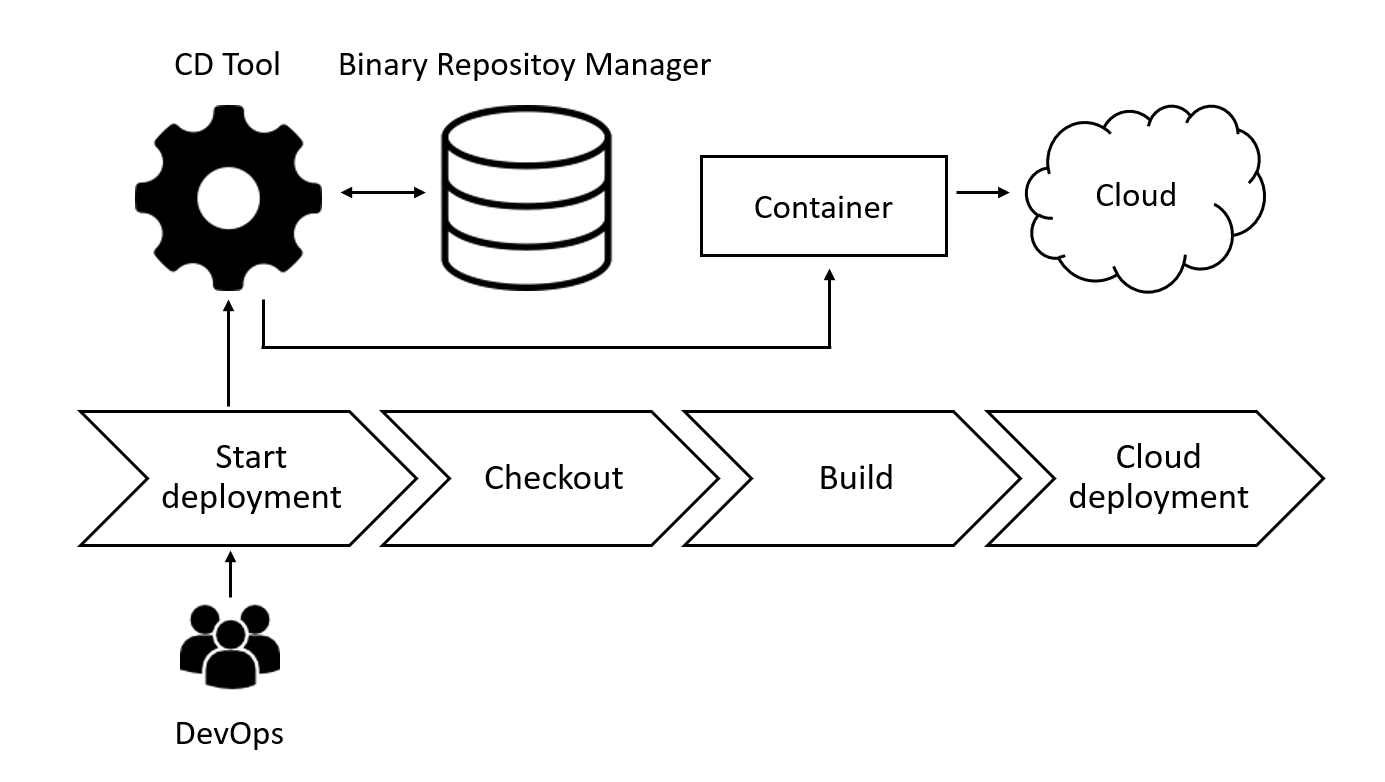
\includegraphics[width=0.8\textwidth]{figures/deployment-process.PNG}
  \caption{ Deployment process~\parencite{Corpancho Villasana 2018}}
  \label{fig:Deployment-process}
\end{figure}

The second part of the defined process is the deployment process as shown in picture \hl{XXX}. The DevOps team triggers manually the deployment process within the CD tool. The tool downloads the latest pushed artifact of the binary repository manager. After downloading the artifact, it build automatically a container out of the artifact. The CD tool pushed then the container to the cloud.

The first approach for a documentation process of the applications running on a cloud-based environment is the establishment of a defined process and a toolchain for building and deploying to the cloud infrastructure. Every application is tracked in the binary repository manager but there is still no integration of the cloud application inventory to the EA tool.

\subsubsection{Monitoring tool integration}

The introduction of a monitoring tool is planned. The reason for establishing a monitoring tool is to gain advantage over the competitors. Monitoring applications allow to retrieve extra information such as individual requests and transactions, resource consumption, reporting and alerting, etc.

The business benefits of monitoring tools for the enterprise are many. One of the benefits is that the enterprise can react quicker to an application failure reducing the revenue loss due to the breakdown of the respective applications or systems. Knowing the failures and obtaining the dependencies from the monitoring tool the enterprise can derive what other systems will be affected by the breakdown. This matches the requirements from the BCM project.

\section{Derived requirements}\label{section:derivedrequirements}

In the previous sections the as-is and target landscape of an insurance company were presented. These sections cover various aspects of the EAD within the studied company. The case study shows different outlooks for future integrations. From the introduced case study, requirements can be derived for for an automated EAD. The following table presents the derived requirements:

\begin{table}[htpb]
  \caption[Automated EAD requirements derived from the case study]{Automated EAD requirements derived the case study}\label{tab:sample}
  \centering
  \begin{tabular}{l l l}
    \toprule
      Id & Requirement\\
    \midrule
      %RC1 & Business Impact Analysis of applications\\
      %RC2 & Data privacy compliance\\
      RC1 & Integration of a PPM tool\\
      RC2 & Integration of other repositories\\
      RC3 & Integration of cloud infrastructure\\
      RC4 & Integration of a monitoring tool\\
    \bottomrule
  \end{tabular}
\end{table}

%\textbf{RC1}: A Business Impact Analysis of applications is not only required by the enterprise, it is also required due to regulations. The enterprise can analyze in case of a sinister what applications are affected and which related systems are implied by a failure. It can quantify the economic impact of failures.

%\textbf{RC2}: Tools have to be compliant with the data privacy regulation. An enterprise needs to know what applications store personal data. 

\textbf{RC3}: The integration of a PPM tool is desired by the enterprise to relate projects to applications.

\textbf{RC4}: An integration of other repositories is required by the enterprise to relate information and propagate information sharing.

\textbf{RC5}: The integration of cloud infrastructure is needed due to a full application inventory required by law and due to strategic decisions as migrating to cloud infrastructure.

\textbf{RC6}: An integration of a monitoring tool is planned at the enterprise to increase the reaction time between the failure of a system and the enterprise. Thus, the monetary impact can reduced.
%BIA
%Migration derivations
%cloud documentation process definition: define process how to document apps.
% automated integration

%top down architecture greefhorst und proper
%architetkruprinzipien meistens auf confluence, copas

%bei architekturüberprüfung gesamt architektur (12factorapp) für konzept oder prototyp

%sozialen druck, transparenz für 12 factors, belt
%aier2018: regeln, steuerung und gehorsam oder "einfach mal laufen lassen
%nudging? - shun long hong

\section{Solution architecture}\label{section:solutionarchitecture}

\section{Prototype evaluation}\label{section:solutionarchitecture}








% !TeX root = ../main.tex
% Add the above to each chapter to make compiling the PDF easier in some editors.

\chapter{Limitations}\label{chapter:conclusion}

\section{Summary}

\section{Future work}
% !TeX root = ../main.tex
% Add the above to each chapter to make compiling the PDF easier in some editors.

\chapter{Conclusion}\label{chapter:Conclusion}

This final chapter of this work presents the summary of this thesis and gives an outlook for further work.

\section{Summary}

This section presents the results for the research questions introduced in section~\ref{section:researchquestions}.

\textbf{RQ1. How to obtain EA relevant information from the runtime behavior of cloud based environments?}
Most cloud infrastructures provide runtime information without the installation of additional monitoring agents. Thus, Shadow IT is prevented. However installing additional monitoring agents unveil further information like the total amount of API requests.  

\textbf{RQ2. How to assign the application landscape to business domains?}
To enable the assignment of the application landscape to the business domains there are two possibilities. The first one is to add the business specific information to a configuration file so the information of the configuration file is used for the assignment. The developers have to manually maintain the configuration file. The second possibility is to integrate the PPM tool in the Build-Deployment pipeline. For this possibility the PPM tool needs to provide the business domain information. This also has to be maintained manually by the developers or the product owners using the PPM tool.

\textbf{RQ3. How to automate the assignment process with an integrated toolchain?}
The automation of the assignment process can be achieved through a configuration file which contains the links to the relevant tools or through name mapping. The usage of the configuration file results in producing further overhead. Therefore the mapping via name is more popular, however the names need to be stable and unique.

\textbf{RQ4. How does a prototype implementation of the automated documentation process of cloud applications look like?}
The prototype implementation of the automated documentation process of cloud applications is explained and illustrated in chapter~\ref{chapter:prototype implementation}.

\section{Future work}

This section presents the possible extensions of the prototype that were not implemented due to time constraints. The future use cases were demanded by the industry partners during the evaluation.

The first additional implementation is to include other cloud environments to enable the transferability to other companies.

During this work the PPM tool was integrated during the build and deployment pipeline to include the business domain information. An further extension would be to include a mapping of business processes and capabilities for an Business Impact Analysis of the applications.

During the evaluation two new code related use cases were requested by the experts. The first use case was the automated verification of the cloud readiness of an application by verifying the 12 factor app criteria. The other use cases was an automated elasticity evaluation through a complete implementation of resilience pattern. To improve both automated verifications an integration a continuous inspection tool to perform automatic reviews with static code analysis would enhance both use cases. A possible tool for this could be Sonarqube\footnote{\url{https://www.sonarqube.org/}}. 

Another requested extension of the prototype is to include an automated Data privacy compliance (GDPR compliance) analysis. Knowing what applications actually store information enables the opportunity to analyze the data that is stored.

To prove that the approach and prototype can automate the EAD of enterprises, access rights to the whole cloud infrastructure needs to be guaranteed and the concept needs to be tested in several pilot projects.

%Solution architecture
%Bild von finale präsi, github


%% !TeX root = ../main.tex
% Add the above to each chapter to make compiling the PDF easier in some editors.

\chapter{Template}\label{chapter:template}

\section{Section}
Citation test~\parencite{latex}.

\subsection{Subsection}

See~\autoref{tab:sample}, \autoref{fig:sample-drawing}, \autoref{fig:sample-plot}, \autoref{fig:sample-listing}.

\begin{table}[htpb]
  \caption[Example table]{An example for a simple table.}\label{tab:sample}
  \centering
  \begin{tabular}{l l l l}
    \toprule
      A & B & C & D \\
    \midrule
      1 & 2 & 1 & 2 \\
      2 & 3 & 2 & 3 \\
    \bottomrule
  \end{tabular}
\end{table}

\begin{figure}[htpb]
  \centering
  % This should probably go into a file in figures/
  \begin{tikzpicture}[node distance=3cm]
    \node (R0) {$R_1$};
    \node (R1) [right of=R0] {$R_2$};
    \node (R2) [below of=R1] {$R_4$};
    \node (R3) [below of=R0] {$R_3$};
    \node (R4) [right of=R1] {$R_5$};

    \path[every node]
      (R0) edge (R1)
      (R0) edge (R3)
      (R3) edge (R2)
      (R2) edge (R1)
      (R1) edge (R4);
  \end{tikzpicture}
  \caption[Example drawing]{An example for a simple drawing.}\label{fig:sample-drawing}
\end{figure}

\begin{figure}[htpb]
  \centering

  \pgfplotstableset{col sep=&, row sep=\\}
  % This should probably go into a file in data/
  \pgfplotstableread{
    a & b    \\
    1 & 1000 \\
    2 & 1500 \\
    3 & 1600 \\
  }\exampleA
  \pgfplotstableread{
    a & b    \\
    1 & 1200 \\
    2 & 800 \\
    3 & 1400 \\
  }\exampleB
  % This should probably go into a file in figures/
  \begin{tikzpicture}
    \begin{axis}[
        ymin=0,
        legend style={legend pos=south east},
        grid,
        thick,
        ylabel=Y,
        xlabel=X
      ]
      \addplot table[x=a, y=b]{\exampleA};
      \addlegendentry{Example A};
      \addplot table[x=a, y=b]{\exampleB};
      \addlegendentry{Example B};
    \end{axis}
  \end{tikzpicture}
  \caption[Example plot]{An example for a simple plot.}\label{fig:sample-plot}
\end{figure}

\begin{figure}[htpb]
  \centering
  \begin{tabular}{c}
  \begin{lstlisting}[language=SQL]
    SELECT * FROM tbl WHERE tbl.str = "str"
  \end{lstlisting}
  \end{tabular}
  \caption[Example listing]{An example for a source code listing.}\label{fig:sample-listing}
\end{figure}

\appendix{}
\chapter{Appendix} \label{chapter:appendix}

%%%%%%%%%%%%%%%%%%%%%%%%%%%%%%%%%%%%%%%%%%%%%%%%%%%%%%%%%%%%
%% Beginning of questionnaire command definitions %%
%%%%%%%%%%%%%%%%%%%%%%%%%%%%%%%%%%%%%%%%%%%%%%%%%%%%%%%%%%%%

%% \Qq = Questionnaire question. Oh, this is just too simple. It helps
%% making it easy to globally change the appearance of questions.
\newcommand{\Qq}[1]{\textbf{#1}}

%% \QO = Circle or box to be ticked. Used both by direct call and by
%% \Qrating and \Qlist.
\newcommand{\QO}{$\Box$}% or: $\ocircle$

%% \Qrating = Automatically create a rating scale with NUM steps, like
%% this: 0--0--0--0--0.
\newcounter{qr}
\newcommand{\Qrating}[1]{\QO\forloop{qr}{1}{\value{qr} < #1}{---\QO}}

%% \Qline = Again, this is very simple. It helps setting the line
%% thickness globally. Used both by direct call and by \Qlines.
\newcommand{\Qline}[1]{\noindent\rule{#1}{0.6pt}}

%% \Qlines = Insert NUM lines with width=\linewith. You can change the
%% \vskip value to adjust the spacing.
\newcounter{ql}
\newcommand{\Qlines}[1]{\forloop{ql}{0}{\value{ql}<#1}{\vskip0em\Qline{\linewidth}}}

%% \Qlist = This is an environment very similar to itemize but with
%% \QO in front of each list item. Useful for classical multiple
%% choice. Change leftmargin and topsep accourding to your taste.
\newenvironment{Qlist}{%
\renewcommand{\labelitemi}{\QO}
\begin{itemize}[leftmargin=1.5em,topsep=-.5em]
}{%
\end{itemize}
}

%% \Qtab = A "tabulator simulation". The first argument is the
%% distance from the left margin. The second argument is content which
%% is indented within the current row.
\newlength{\qt}
\newcommand{\Qtab}[2]{
\setlength{\qt}{\linewidth}
\addtolength{\qt}{-#1}
\hfill\parbox[t]{\qt}{\raggedright #2}
}

%% \Qitem = Item with automatic numbering. The first optional argument
%% can be used to create sub-items like 2a, 2b, 2c, ... The item
%% number is increased if the first argument is omitted or equals 'a'.
%% You will have to adjust this if you prefer a different numbering
%% scheme. Adjust topsep and leftmargin as needed.
\newcounter{itemnummer}
\newcommand{\Qitem}[2][]{% #1 optional, #2 notwendig
\ifthenelse{\equal{#1}{}}{\stepcounter{itemnummer}}{}
\ifthenelse{\equal{#1}{a}}{\stepcounter{itemnummer}}{}
\begin{enumerate}[topsep=2pt,leftmargin=2.8em]
\item[\textbf{\arabic{itemnummer}#1.}] #2
\end{enumerate}
}

%% \QItem = Like \Qitem but with alternating background color. This
%% might be error prone as I hard-coded some lengths (-5.25pt and
%% -3pt)! I do not yet understand why I need them.
\definecolor{bgodd}{rgb}{0.8,0.8,0.8}
\definecolor{bgeven}{rgb}{0.9,0.9,0.9}
\newcounter{itemoddeven}
\newlength{\gb}
\newcommand{\QItem}[2][]{% #1 optional, #2 notwendig
\setlength{\gb}{\linewidth}
\addtolength{\gb}{-5.25pt}
\ifthenelse{\equal{\value{itemoddeven}}{0}}{%
\noindent\colorbox{bgeven}{\hskip-3pt\begin{minipage}{\gb}\Qitem[#1]{#2}\end{minipage}}%
\stepcounter{itemoddeven}%
}{%
\noindent\colorbox{bgodd}{\hskip-3pt\begin{minipage}{\gb}\Qitem[#1]{#2}\end{minipage}}%
\setcounter{itemoddeven}{0}%
}
}

%%%%%%%%%%%%%%%%%%%%%%%%%%%%%%%%%%%%%%%%%%%%%%%%%%%%%%%%%%%%
%% End of questionnaire command definitions %%
%%%%%%%%%%%%%%%%%%%%%%%%%%%%%%%%%%%%%%%%%%%%%%%%%%%%%%%%%%%%

\section{Evaluation questionnaire}

\subsubsection{1. General data}

\Qq{Company}: \Qline{4cm} \Qq{Date and time}: \Qline{4cm} \\
\Qq{Interviewer}: \Qline{4cm} \Qq{Questionnaire-Nr.}: \Qline{4cm} \\
\Qq{Years of experience}: \Qline{4cm} \Qq{Industry sector}: \Qline{4cm}

\Qitem{\Qq{Which of the below roles are applicable for you?}\\
\QO Enterprise Architect  \QO Product Owner  \QO DevOps  \QO Other: \Qline{3cm}
}
\Qitem{\Qq{It is a lot of effort to document the IT landscape of your company}\\
\QO Strongly agree  \QO agree  \QO disagree  \QO Strongly disagree
}

\Qitem{\Qq{The information in the EA tool is outdated}\\
\QO Yes  \QO No
}
\Qitem{\Qq{Does your company have an automated process for documenting the EA?}\\
\QO Yes  \QO No
}
\Qitem{\Qq{If your company has an automated process for documenting the EA, please describe the process:}
\Qlines{2}
}

\Qitem{\Qq{Does your company run applications/services in a cloud-based environment?}\\
\QO Yes  \QO No
}

\Qitem{\Qq{Does your company consider migrating legacy systems into a cloud-based environment?}\\
\QO Yes  \QO No
}

\subsubsection{2. Agile methodologies}

\Qitem{\Qq{Does your company use a Continuous Delivery approach?}\\
\QO Yes  \QO No
}

\Qitem{\Qq{Who collects the EA information of a new developed application/service for the EA Tool?}\\
\QO Enterprise Architect  \QO Product Owner  \QO DevOps  \QO Other: \Qline{3cm}
}

\Qitem{\Qq{Do you use any of the above mentioned information sources to retrieve EA relevant information?}\\
\QO Network scanners and monitors  \QO CMDB  \QO PPM  \QO ESB  \QO Other: \Qline{2cm}
}

\Qitem{\Qq{Do you use any of the above mentioned information sources to retrieve EA relevant information?}\\
\QO Runtime environment  \QO Jira  \QO Github  \QO Jenkins  \QO Wiki
}

\Qitem{\Qq{Do you think this information sources could contain relevant EA information? Why?}
\Qlines{2}
}

\Qitem{\Qq{How do you collect this information?}
\Qlines{2}
}

\Qitem{\Qq{Does your company have an established toolchain for the development pipeline?}\\
\QO Yes  \QO No
}

\Qitem{\Qq{Do you think an established toolchain improve the process of EA documentation?Why?}\\
\QO Yes  \QO No
\Qlines{2}
}


\Qitem{\Qq{Imposing the team to incorporate a pipeline-script in the repository is easy to establish}\\
\QO Strongly agree  \QO agree  \QO disagree  \QO Strongly disagree
}

\Qitem{\Qq{Imposing the team to use a predefined toolchain for the application development is easy to establish}\\
\QO Strongly agree  \QO agree  \QO disagree  \QO Strongly disagree
}

\Qitem{\Qq{How do you determine an application owner?}\\
\Qlines{2}
}

\Qitem{\Qq{Do you follow any guidelines when developing a new product?}\\
\Qlines{2}
}

\subsubsection{3. Cloud environments}

\Qitem{\Qq{Does your company use any technologies for automating the EA documentation process?}\\
\QO Yes  \QO No
}

\Qitem{\Qq{How does your company collect the applications running in a cloud-based environment?}\\
\QO Yes  \QO No
}

\Qitem{\Qq{Does your company have any architecture guidelines for cloud applications?}\\
\QO Yes  \QO No
}

\Qitem{\Qq{Are you familiar with the 12-factor-app criteria for determining if an application/product is cloud-ready?}\\
\QO Yes  \QO No
}

\Qitem{\Qq{Do you use any technologies for monitoring applications?}\\
\QO Yes  \QO No
}

\Qitem{\Qq{If yes, please give a short answer regarding the technologies used for monitoring the applications/services:}\\
\Qlines{2}
}

\subsubsection{4. Tool Evaluation}

\Qitem{\Qq{The presented prototype covers different views for the different stakeholders such as product owners, enterprise architects and devops-teams}\\
\QO Strongly agree  \QO agree  \QO disagree  \QO Strongly disagree
}

\Qitem{\Qq{The presented prototype enables a federated approach linking the tools used during an application development pipeline}\\
\QO Strongly agree  \QO agree  \QO disagree  \QO Strongly disagree
}

\Qitem{\Qq{The following information displayed in the general section of the detailed view of an application/service is useful}\\
\QO Status  \QO Name  \QO Description  \QO Domain  \QO Subdomain \\
\QO Product  \QO Owner  \QO Json link  \QO Changes  \QO Additional information
}

\Qitem{\Qq{The following information displayed in the general section of the detailed view of an application/service is NOT useful.Why?}\\
\QO Status  \QO Name  \QO Description  \QO Domain  \QO Subdomain \\
\QO Product  \QO Owner  \QO Json link  \QO Changes  \QO Additional information
\Qlines{2}
}

\Qitem{\Qq{I would like to see the following information displayed in the general section:}
\Qlines{2}
}

\Qitem{\Qq{The following information in the runtime section is useful}\\
\QO Instances  \QO Ram  \QO CPU  \QO Disk  \QO Host
}

\Qitem{\Qq{The following information in the runtime section is NOT useful. Why?}\\
\QO Instances  \QO Ram  \QO CPU  \QO Disk  \QO Host
\Qlines{2}
}

\Qitem{\Qq{I would like to see the following information displayed in the runtime section:}
\Qlines{2}
}

\Qitem{\Qq{The following information displayed is the metrics section is useful}\\
\QO URL  \QO Prometheus metrics endpoint  \QO Response time
}

\Qitem{\Qq{The following information displayed is the metrics section is NOT useful. Why?}\\
\QO URL  \QO Prometheus metrics endpoint  \QO Response time
\Qlines{2}
}

\Qitem{\Qq{I would like to see the following information displayed in the metrics section:}
\Qlines{2}
}

\Qitem{\Qq{The information displayed in the Application/Services section is useful.If no, why?}\\
\QO Yes  \QO No
\Qlines{2}
}

\Qitem{\Qq{The information displayed in the software dependencies section is useful. Why?}\\
\QO Yes  \QO No
\Qlines{2}
}

\Qitem{\Qq{The following information in the Jira monitoring section is useful:}\\
\QO Total issues  \QO Open issues  \QO Components  \QO Project progress
}

\Qitem{\Qq{The following information in the Jira monitoring section is NOT useful. Why?}\\
\QO Total issues  \QO Open issues  \QO Components  \QO Project progress
\Qlines{2}
}

\Qitem{\Qq{I would like to see the following information displayed in the jira  section:}
\Qlines{2}
}

\Qitem{\Qq{The following information in the github monitoring section is useful:}\\
\QO Contributors  \QO Lines of Code  \QO Commit activity
}

\Qitem{\Qq{The following information in the github monitoring section is NOT useful. Why?}\\
\QO Contributors  \QO Lines of Code  \QO Commit activity
\Qlines{2}
}

\Qitem{\Qq{What information would you like to see in the Github monitoring section regarding the repository of the application?}
\Qlines{2}
}

\Qitem{\Qq{The following information displayed in the Jenkins job monitoring section is useful:}\\
\QO Build number  \QO Duration  \QO Estimated duration  \QO Result  \QO Timestamp
}

\Qitem{\Qq{The following information displayed in the Jenkins job monitoring section is NOT useful. Why?}\\
\QO Build number  \QO Duration  \QO Estimated duration  \QO Result  \QO Timestamp
\Qlines{2}
}

\Qitem{\Qq{An automated test 12-factor evaluation of the application/service is helpful to evaluate if the application/service is cloud-ready:}\\
\QO Yes  \QO No
}

\Qitem{\Qq{An automated test of the resilience pattern is helpful to determine the elasticity of an application/service:}\\
\QO Yes  \QO No
}

\Qitem{\Qq{An integration of the architecture belt tool would improve the governance monitoring section:}\\
\QO Yes  \QO No
}

\Qitem{\Qq{The presented sections represent relevant EA information sources}\\
\QO Yes  \QO No
}

\Qitem{\Qq{Would you include other information sources?}\\
\QO Yes  \QO No
} 

\Qitem{\Qq{If yes please describe briefly why:}\\
\Qlines{2}
} 

\Qitem{\Qq{The visualizations displayed in the visualizations tab is useful:}\\
\QO Yes  \QO No
} 

\Qitem{\Qq{I would like to see the following visualizations:}
\Qlines{2}
}

\Qitem{\Qq{Other comments:}
\Qlines{3}
}

\subsubsection{5. Overall}

\Qitem{\Qq{The presented process will automate the EA documentation of applications/services running on a cloud-based environment}\\
\QO Strongly agree  \QO agree  \QO disagree  \QO Strongly disagree
}

\Qitem{\Qq{Overall score of the tool: Being 5 the best}\\
\QO 1  \QO 2  \QO 3  \QO 4  \QO 5
}


\microtypesetup{protrusion=true}
\printbibliography{}

\appendix{}


\end{document}
